% !TeX spellcheck = de-DE
% !TeX encoding = utf8
% !TeX program = lualatex
% !TeX TXS-program:compile = txs:///lualatex/[--shell-escape]
% !BIB program = biber
% -*- coding:utf-8 mod:LaTeX -*-

% vv  scroll down to line 200 for content  vv


\let\ifdeutsch\iftrue
\let\ifenglisch\iffalse
% EN: This file is loaded before the \documentclass command in the main document

% EN: The following package allows \\ at the title page
%     For more information see https://github.com/latextemplates/scientific-thesis-cover/issues/4
\RequirePackage{kvoptions-patch}

\ifenglisch
  \PassOptionsToClass{numbers=noenddot}{scrbook}
\else
  %()Aus scrguide.pdf - der Dokumentation von KOMA-Script)
  %Nach DUDEN steht in Gliederungen, in denen ausschließlich arabische Ziffern für die Nummerierung
  %verwendet werden, am Ende der Gliederungsnummern kein abschließender Punkt
  %(siehe [DUD96, R3]). Wird hingegen innerhalb der Gliederung auch mit römischen Zahlen
  %oder Groß- oder Kleinbuchstaben gearbeitet, so steht am Ende aller Gliederungsnummern ein
  %abschließender Punkt (siehe [DUD96, R4])
  \PassOptionsToClass{numbers=autoendperiod}{scrbook}
\fi

% Warns about outdated packages and missing caption declarations
% See https://www.ctan.org/pkg/nag
\RequirePackage[l2tabu, orthodox]{nag}

%DE: Neue deutsche Trennmuster
%    Siehe http://www.ctan.org/pkg/dehyph-exptl und http://projekte.dante.de/Trennmuster/WebHome
%    Nur für pdflatex, nicht für lualatex
\RequirePackage{ifluatex}
\ifluatex
  % do not load anything
\else
  \ifdeutsch
    \RequirePackage[ngerman=ngerman-x-latest]{hyphsubst}
  \fi
\fi

\documentclass[
  % fontsize=11pt is the standard
  a4paper,  % Standard format - only KOMAScript uses paper=a4 - https://tex.stackexchange.com/a/61044/9075
  twoside,  % we are optimizing for both screen and two-side printing. So the page numbers will jump, but the content is configured to stay in the middle (by using the geometry package)
  bibliography=totoc,
  %               idxtotoc,   %Index ins Inhaltsverzeichnis
  %               liststotoc, %List of X ins Inhaltsverzeichnis, mit liststotocnumbered werden die Abbildungsverzeichnisse nummeriert
  headsepline,
  cleardoublepage=empty,
  parskip=half,
  %               draft    % um zu sehen, wo noch nachgebessert werden muss - wichtig, da Bindungskorrektur mit drin
  draft=false
]{scrbook}
% !TeX encoding = utf8
% -*- coding:utf-8 mod:LaTeX -*-

% EN: This file includes basic packages and sets options. The order of package
%     loading is important
% DE: In dieser Datei werden zuerst die benoetigten Pakete eingebunden und
%     danach diverse Optionen gesetzt. Achtung Reihenfolge ist entscheidend!


%%%
% EN: Styleguide:
% - English comments are prefixed with "EN", German comments are prefixed with "DE"
% - Prefixed headings define the language for the subsequent paragraphs
% - It is tried to organize packages in blocks. One block starts with %%%, then
%   % <heading>, then the options and more text. % followed by %%% end a block.
%
% DE: Styleguide:
%
% Ein sehr kleiner Styleguide. Packages werden in Blöcken organisiert.
% Ein Block beginnt mit drei % in einer Zeile, dann % <Blocküberschrift>, dann
% eine Liste der möglichen Optionen und deren Einstellungen, Gründe und Kommentare
% eine % Zeile in der sonst nichts steht und dann wieder %%% in einer Zeile.
%
% Zwischen zwei Blöcken sind 2 Leerzeilen!
% Zu jedem Paket werden soviele Optionen wie möglich/nötig angegeben
%
%%%


%%%
% EN: Enable copy and paste of text from the PDF
%     Only required for pdflatex. It "just works" in the case of lualatex.
%     mmap enables mathematical symbols, but does not work with the newtx font set
%     See: https://tex.stackexchange.com/a/64457/9075
%     Other solutions outlined at http://goemonx.blogspot.de/2012/01/pdflatex-ligaturen-und-copynpaste.html and http://tex.stackexchange.com/questions/4397/make-ligatures-in-linux-libertine-copyable-and-searchable
%     Trouble shooting outlined at https://tex.stackexchange.com/a/100618/9075
\ifluatex
\else
  \usepackage{cmap}
\fi
%%%


%%%
% EN: File encoding
% DE: Codierung
%     Wir sind im 21 Jahrhundert, utf-8 löst so viele Probleme.
%
% Mit UTF-8 funktionieren folgende Pakete nicht mehr. Bitte beachten!
%   * fancyvrb mit §
%   * easylist -> http://www.ctan.org/tex-archive/macros/latex/contrib/easylist/
\ifluatex
  % EN: See https://tex.stackexchange.com/a/158517/9075
  %     Not required, because of usage of fontspec package
  %\usepackage[utf8]{luainputenc}
\else
  \usepackage[utf8]{inputenc}
\fi
%
%%%

%%%
% DE: Parallelbetrieb tex4ht und pdflatex
\makeatletter
\@ifpackageloaded{tex4ht}{
  \def\iftex4ht{\iftrue}
}{
  \def\iftex4ht{\iffalse}
}
\makeatother
%%%


%%%
% EN: Defintion of colors
% DE: Farbdefinitionen
\usepackage[hyperref,dvipsnames]{xcolor}
%

%%%
% EN: Required for custom acronyms/glossaries style.
%     Left aligned Columns in tables with fixed width.
%     See http://tex.stackexchange.com/questions/91566/syntax-similar-to-centering-for-right-and-left
\usepackage{ragged2e}
%%%

%%%
% EN: Abbreviations
% DE: Abkürzungsverzeichnis
%
% DE: Wichtig, ansonsten erscheint "No room for a new \write"
\usepackage{scrwfile}
% DE: siehe http://www.dickimaw-books.com/cgi-bin/faq.cgi?action=view&categorylabel=glossaries#glsnewwriteexceeded
\usepackage[acronym,indexonlyfirst,nomain]{glossaries}
\ifdeutsch
  \renewcommand*{\acronymname}{Abkürzungsverzeichnis}
\else
  \renewcommand*{\acronymname}{List of Abbreviations}
\fi
\renewcommand*{\glsgroupskip}{}
%
% EN: Removed Glossarie as a table as a quick fix to get the template working again
%     See http://tex.stackexchange.com/questions/145579/how-to-print-acronyms-of-glossaries-into-a-table
%
\makenoidxglossaries
%%%


%%%
% EN: Support for language-specific hyphenation
% DE: Neue deutsche Rechtschreibung und Literatur statt "Literature"
%     Die folgende Einstellung ist der Nachfolger von ngerman.sty
\ifdeutsch
  % DE: letzte Sprache ist default, Einbindung von "american" ermöglicht \begin{otherlanguage}{amercian}...\end{otherlanguage} oder \foreignlanguage{american}{Text in American}
  %     Siehe auch http://tex.stackexchange.com/a/50638/9075
  \usepackage[american,ngerman]{babel}
  % Ein "abstract" ist eine "Kurzfassung", keine "Zusammenfassung"
  \addto\captionsngerman{%
    \renewcommand\abstractname{Kurzfassung}%
  }
  \ifluatex
    % EN: conditionally disable ligatures. See https://github.com/latextemplates/scientific-thesis-template/issues/54
    %     for a discussion
    \usepackage[ngerman]{selnolig}
  \fi
\else
  % EN: Set English as language and allow to write hyphenated"=words
  %     `american`, `english` and `USenglish` are synonyms for babel package (according to https://tex.stackexchange.com/questions/12775/babel-english-american-usenglish).
  %      "english" has to go last to set it as default language
  \usepackage[ngerman,english]{babel}
  % EN: Hint by http://tex.stackexchange.com/a/321066/9075 -> enable "= as dashes
  \addto\extrasenglish{\languageshorthands{ngerman}\useshorthands{"}}
  \ifluatex
    % EN: conditionally disable ligatures. See https://github.com/latextemplates/scientific-thesis-template/issues/54
    %     for a discussion
    \usepackage[english]{selnolig}
  \fi
\fi
%
%%%


%%%
% EN: For easy quotations: \enquote{text}
%     This package is very smart when nesting is applied, otherwise textcmds (see below) provides a shorter command
% DE:  Anführungszeichen
%      Zitate in \enquote{...} setzen, dann werden automatisch die richtigen Anführungszeichen verwendet.
\usepackage{csquotes}
%%%


%%%
% EN: For even easier quotations: \qq{text}.
%     Is not smart in the case of nesting, but good enough for the most cases
\usepackage{textcmds}
\ifdeutsch
  % EN: German quotes are different. So do not use the English quotes, but the ones provided by the csquotes package.
  \renewcommand{\qq}[1]{\enquote{#1}}
\fi
%%%


%%%
% EN: extended enumarations
% DE: erweitertes Enumerate
\usepackage{paralist}
%
%%%


%%%
% DE: fancyheadings (nicht nur) fuer koma
\usepackage[automark]{scrlayer-scrpage}
%
%%%


%%%
% EN: Mathematics
% DE: Mathematik
%
% DE: Viele Mathematik-Sachen. Siehe https://texdoc.net/pkg/amsmath
\usepackage{amsmath}
% EN: Options must be passed this way, otherwise it does not work with glossaries
\PassOptionsToPackage{fleqn,leqno}{amsmath}
% DE: fleqn (=Gleichungen linksbündig platzieren) funktioniert nicht direkt. Es muss noch ein Patch gemacht werden:
%\addtolength\mathindent{1em}%work-around ams-math problem with align and 9 -> 10. Does not work with glossaries, No visual changes.
% EN: Fixes bugs in AMS math
\usepackage{mathtools}
%
% EN: For theorems, replacement for amsthm
\usepackage[amsmath,hyperref]{ntheorem}
\theorempreskipamount 2ex plus1ex minus0.5ex
\theorempostskipamount 2ex plus1ex minus0.5ex
\theoremstyle{break}
\newtheorem{definition}{Definition}[section]
%
%%%


%%%
% DE: Intelligentes Leerzeichen um hinter Abkürzungen die richtigen Abstände zu erhalten, auch leere.
%     Siehe commands.tex \gq{}
\usepackage{xspace}
%DE: Macht \xspace und \enquote kompatibel
\makeatletter
\xspaceaddexceptions{\grqq \grq \csq@qclose@i \} }
\makeatother
%
%%%


%%%
% EN: Package for the appendix
% DE: Anhang
\usepackage{appendix}
%[toc,page,title,header]
%
%%%

%%%
% EN: Graphics
% DE: Grafikeinbindungen
%
% EN: The parameter "pdftex" is not required
\usepackage{graphicx}
\graphicspath{{\getgraphicspath}}
\newcommand{\getgraphicspath}{graphics/}
%
%%%


%%%
% EN: Enables inclusion of SVG graphics - 1:1 approach
%    This is NOT the approach of https://ctan.org/pkg/svg-inkscape,
%     which allows text in SVG to be typeset using LaTeX
%     We just include the SVG as is.
\usepackage{epstopdf}
\epstopdfDeclareGraphicsRule{.svg}{pdf}{.pdf}{%
  inkscape -z -D --file=#1 --export-pdf=\OutputFile
}
%
%%%


%%%
% EN: Enables inclusion of SVG graphics - text-rendered-with-LaTeX-approach
%     This is the approach of https://ctan.org/pkg/svg-inkscape,
\newcommand{\executeiffilenewer}[3]{%
  \IfFileExists{#2}
  {
    %\message{file #2 exists}
    \ifnum\pdfstrcmp{\pdffilemoddate{#1}}%
      {\pdffilemoddate{#2}}>0%
      {\immediate\write18{#3}}
    \else
      {%\message{file up to date #2}
      }
    \fi%
  }{
    %\message{file #2 doesn't exist}
    %\message{argument: #3}
    %\immediate\write18{echo "test" > xoutput.txt}
    \immediate\write18{#3}
  }
}
\newcommand{\includesvg}[1]{%
  \executeiffilenewer{#1.svg}{#1.pdf}%
  {
    inkscape -z -D --file=\getgraphicspath#1.svg %
    --export-pdf=\getgraphicspath#1.pdf --export-latex}%
  \input{\getgraphicspath#1.pdf_tex}%
}


%%%
% EN: Enable typesetting values with SI units.
\ifdeutsch
  \usepackage[mode=text,group-four-digits]{siunitx}
  \sisetup{locale=DE}
\else
  \usepackage[mode=text,group-four-digits,group-separator={,}]{siunitx}
  \sisetup{locale=US}
\fi
%%%

%%%
% EN: Extensions for tables
% DE: Tabellenerweiterungen
\usepackage{array} %increases tex's buffer size and enables ``>'' in tablespecs
\usepackage{longtable}
\usepackage{dcolumn} %Aligning numbers by decimal points in table columns
\ifdeutsch
  \newcolumntype{d}[1]{D{.}{,}{#1}}
\else
  \newcolumntype{d}[1]{D{.}{.}{#1}}
\fi
\setlength{\extrarowheight}{1pt}
%%%

%%%
% Eine Zelle, die sich über mehrere Zeilen erstreckt.
% Siehe Beispieltabelle in Kapitel 2
\usepackage{multirow}
%
%%%

%%%
%Fuer Tabellen mit Variablen Spaltenbreiten
%\usepackage{tabularx}
%\usepackage{tabulary}
%
%%%


%%%
% EN: Links behave as they should. Enables "\url{...}" for URL typesettings.
%     Allow URL breaks also at a hyphen, even though it might be confusing: Is the "-" part of the address or just a hyphen?
%     See https://tex.stackexchange.com/a/3034/9075.
% DE: Links verhalten sich so, wie sie sollen
%     Zeilenumbrüche bei URLs auch bei Bindestrichen erlauben, auch wenn es verwirrend sein könnte: Gehört der Bindestrich zur URL oder ist es ein Trennstrich?
%     Siehe https://tex.stackexchange.com/a/3034/9075.
\usepackage[hyphens]{url}
%
%  EN: When activated, use text font as url font, not the monospaced one.
%      For all options see https://tex.stackexchange.com/a/261435/9075.
% \urlstyle{same}
%
% EN: Hint by http://tex.stackexchange.com/a/10419/9075.
\makeatletter
\g@addto@macro{\UrlBreaks}{\UrlOrds}
\makeatother
%
%%%


%%%
% Index über Begriffe, Abkürzungen
%\usepackage{makeidx} makeidx ist out -> http://xindy.sf.net verwenden
%
%%%

%%%
%lustiger Hack fuer das Abkuerzungsverzeichnis
%nach latex durchlauf folgendes ausfuehren
%makeindex ausarbeitung.nlo -s nomencl.ist -o ausarbeitung.nls
%danach nochmal latex
%\usepackage{nomencl}
%    \let\abk\nomenclature %Deutsche Ueberschrift setzen
%          \renewcommand{\nomname}{List of Abbreviations}
%        %Punkte zw. Abkuerzung und Erklaerung
%          \setlength{\nomlabelwidth}{.2\hsize}
%          \renewcommand{\nomlabel}[1]{#1 \dotfill}
%        %Zeilenabstaende verkleinern
%          \setlength{\nomitemsep}{-\parsep}
%    \makenomenclature
%
%%%

%%%
% EN: Logic for TeX - enables if-then-else in commands
% DE: Logik für TeX
%     FÜr if-then-else @ commands.tex
\usepackage{ifthen}
%
%%%


%%%
% EN: Code Listings
% DE: Listings
\usepackage{listings}
\lstset{language=XML,
  showstringspaces=false,
  extendedchars=true,
  basicstyle=\footnotesize\ttfamily,
  commentstyle=\slshape,
  % DE: Original: \rmfamily, damit werden die Strings im Quellcode hervorgehoben. Zusaetzlich evtl.: \scshape oder \rmfamily durch \ttfamily ersetzen. Dann sieht's aus, wie bei fancyvrb
  stringstyle=\ttfamily,
  breaklines=true,
  breakatwhitespace=true,
  % EN: alternative: fixed
  columns=flexible,
  numbers=left,
  numberstyle=\tiny,
  basewidth=.5em,
  xleftmargin=.5cm,
  % aboveskip=0mm, %DE: deaktivieren, falls man lstlistings direkt als floating object benutzt (\begin{lstlisting}[float,...])
  % belowskip=0mm, %DE: deaktivieren, falls man lstlistings direkt als floating object benutzt (\begin{lstlisting}[float,...])
  captionpos=b
}

\ifluatex
\else
  % EN: Enable UTF-8 support - see https://tex.stackexchange.com/q/419327/9075
  \usepackage{listingsutf8}
  \lstset{inputencoding=utf8/latin1}
\fi

\ifdeutsch
  \renewcommand{\lstlistlistingname}{Verzeichnis der Listings}
\fi
%
%%%


%%%
% EN: Alternative to listings could be fancyvrb. Can be used together.
% DE: Alternative zu Listings ist fancyvrb. Kann auch beides gleichzeitig benutzt werden.
\usepackage{fancyvrb}
%
%EN: Font size for the normal text
%DE: Groesse fuer den Fliesstext. Falls deaktiviert: \normalsize
%\fvset{fontsize=\small}
%
%DE: Somit kann im Text ganz einfach §verbatim§ text gesetzt werden.
%    Disabled, because UTF-8 does not work any more and lualatex causes issues
%\DefineShortVerb{\§}
%
%EN: Shrink font size of listings
\RecustomVerbatimEnvironment{Verbatim}{Verbatim}{fontsize=\footnotesize}
\RecustomVerbatimCommand{\VerbatimInput}{VerbatimInput}{fontsize=\footnotesize}
%
%EN: Hack for fancyvrb based on http://newsgroups.derkeiler.com/Archive/Comp/comp.text.tex/2008-12/msg00075.html
%EN: Change of the solution: \Vref somehow collidated with cleveref/varioref as the output of \Vref{} was "Abschnitt 4.3 auf Seite 85"; therefore changed to \myVref -- so completely removed
\newcommand{\Vlabel}[1]{\label[line]{#1}\hypertarget{#1}{}}
\newcommand{\lref}[1]{\hyperlink{#1}{\FancyVerbLineautorefname~\ref*{#1}}}
%
%%%


%%%
% EN: Tunings of captions for floats, listings, ...
% DE: Bildunterschriften bei floats genauso formatieren wie bei Listings
%     Anpassung wird unten bei den newfloat-Deklarationen vorgenommen
%     https://www.ctan.org/pkg/caption2 is superseeded by this package.
\usepackage{caption}
%
%%%


%%%
% EN: Provides rotating figures, where the PDF page is also turned
% DE: Ermoeglicht es, Abbildungen um 90 Grad zu drehen
%     Alternatives Paket: rotating Allerdings wird hier nur das Bild gedreht, während bei lscape auch die PDF-Seite gedreht wird.
%     Das Paket lscape dreht die Seite auch nicht
\usepackage{pdflscape}
%
%%%


%%%
%EN: Required for proper environments of fancyvrb and lstlistings
%    There is also the newfloat pacakge (recommended by minted), but we currently have no expericene with that
%DE: Wird für fancyvrb und für lstlistings verwendet
\usepackage{float}
%
% EN: Alternative to float package
%\usepackage{floatrow}
%DE: zustäzlich für den Paramter [H] = Floats WIRKLICH da wo sie deklariert wurden paltzieren - ganz ohne Kompromisse
%    floatrow ist der Nachfolger von float
%    Allerdings macht floatrow in manchen Konstellationen Probleme. Deshalb ist das Paket deaktiviert.
%
% EN: See http://www.tex.ac.uk/cgi-bin/texfaq2html?label=floats
% DE: floats IMMER nach einer Referenzierung platzieren
%\usepackage{flafter}
%%%


%%%
% EN: For nested figures
% DE: Fuer Abbildungen innerhalb von Abbildungen
%     Ersetzt die Pakete subfigure und subfig - siehe https://tex.stackexchange.com/a/13778/9075
\usepackage[hypcap=true]{subcaption}
%
%%%


%%%
% EN: Extended support for footnotes
% DE: Fußnoten
%
%\usepackage{dblfnote}  %Zweispaltige Fußnoten
%
% Keine hochgestellten Ziffern in der Fußnote (KOMA-Script-spezifisch):
%\deffootnote[1.5em]{0pt}{1em}{\makebox[1.5em][l]{\bfseries\thefootnotemark}}
%
% Abstand zwischen Fußnoten vergrößern:
%\setlength{\footnotesep}{.85\baselineskip}
%
% EN: Following command disables the separting line of the footnote
% DE: Folgendes Kommando deaktiviert die Trennlinie zur Fußnote
%\renewcommand{\footnoterule}{}
%
\addtolength{\skip\footins}{\baselineskip} % Abstand Text <-> Fußnote
%
% Fußnoten immer ganz unten auf einer \raggedbottom-Seite
% fnpos kommt aus dem yafoot package
\usepackage{fnpos}
\makeFNbelow
\makeFNbottom
%
%%%


%%%
% EN: Variable page heights
% DE: Variable Seitenhöhen zulassen
\raggedbottom
%
%%%


%%%
% Falls die Seitenzahl bei einer Referenz auf eine Abbildung nur dann angegeben werden soll,
% falls sich die Abbildung nicht auf der selben Seite befindet...
\iftex4ht
  %tex4ht does not work well with vref, therefore we emulate vref behavior
  \newcommand{\vref}[1]{\ref{#1}}
\else
  \ifdeutsch
    \usepackage[ngerman]{varioref}
  \else
    \usepackage{varioref}
  \fi
\fi
%%%

%%%
% EN: More beautiful tables if one uses \toprule, \midrule, \bottomrule
% DE: Noch schoenere Tabellen als mit booktabs mit http://www.zvisionwelt.de/downloads.html
\usepackage{booktabs}
%
%\usepackage[section]{placeins}
%
%%%


%%%
% EN: Graphs and Automata
%
% TODO: Since version 3.0 (2013-10-01), it supports pdflatex via the auto-pst-pdf package
%       Requires -shell-escape
%\usepackage{gastex}
%%%


%%%
%
%\usepackage{multicol}
%\usepackage{setspace} % kollidiert mit diplomarbeit.sty
%%%


%%%
%biblatex statt bibtex
\usepackage[
  backend       = biber, %biber does not work with 64x versions alternative: bibtex8
  %minalphanames only works with biber backend
  sortcites     = true,
  bibstyle      = alphabetic,
  citestyle     = alphabetic,
  giveninits    = true,
  useprefix     = false, %"von, van, etc." will be printed, too. See below.
  minnames      = 1,
  minalphanames = 3,
  maxalphanames = 4,
  maxbibnames   = 99,
  maxcitenames  = 2,
  natbib        = true,
  eprint        = true,
  url           = true,
  doi           = true,
  isbn          = true,
  backref       = true]{biblatex}

% enable more breaks at URLs. See https://tex.stackexchange.com/a/134281.
\setcounter{biburllcpenalty}{7000}
\setcounter{biburlucpenalty}{8000}

\bibliography{bibliography}
%\addbibresource[datatype=bibtex]{bibliography.bib}

%Do not put "vd" in the label, but put it at "\citeauthor"
%Source: http://tex.stackexchange.com/a/30277/9075
\makeatletter
\AtBeginDocument{\toggletrue{blx@useprefix}}
\AtBeginBibliography{\togglefalse{blx@useprefix}}
\makeatother

%Thin spaces between initials
%http://tex.stackexchange.com/a/11083/9075
\renewrobustcmd*{\bibinitdelim}{\,}

%Keep first and last name together in the bibliography
%http://tex.stackexchange.com/a/196192/9075
\renewcommand*\bibnamedelimc{\addnbspace}
\renewcommand*\bibnamedelimd{\addnbspace}

%Replace last "and" by comma in bibliography
%See http://tex.stackexchange.com/a/41532/9075
\AtBeginBibliography{%
  \renewcommand*{\finalnamedelim}{\addcomma\space}%
}

\DefineBibliographyStrings{ngerman}{
  backrefpage  = {zitiert auf S\adddot},
  backrefpages = {zitiert auf S\adddot},
  andothers    = {et\ \addabbrvspace al\adddot},
  %Tipp von http://www.mrunix.de/forums/showthread.php?64665-biblatex-Kann-%DCberschrift-vom-Inhaltsverzeichnis-nicht-%E4ndern&p=293656&viewfull=1#post293656
  bibliography = {Literaturverzeichnis}
}

%enable hyperlinked author names when using \citeauthor
%source: http://tex.stackexchange.com/a/75916/9075
\DeclareCiteCommand{\citeauthor}
{\boolfalse{citetracker}%
  \boolfalse{pagetracker}%
  \usebibmacro{prenote}}
{\ifciteindex
  {\indexnames{labelname}}
  {}%
  \printtext[bibhyperref]{\printnames{labelname}}}
{\multicitedelim}
{\usebibmacro{postnote}}

%natbib compatibility
%\newcommand{\citep}[1]{\cite{#1}}
%\newcommand{\citet}[1]{\citeauthor{#1} \cite{#1}}
%Beginning of sentence - analogous to cleveref - important for names such as "zur Muehlen"
%\newcommand{\Citep}[1]{\cite{#1}}
%\newcommand{\Citet}[1]{\Citeauthor{#1} \cite{#1}}
%%%


%%%
% DE: Blindtext. Paket "blindtext" ist fortgeschritterner als "lipsum" und kann auch Mathematik im Text (http://texblog.org/2011/02/26/generating-dummy-textblindtext-with-latex-for-testing/)
%     kantlipsum (https://www.ctan.org/tex-archive/macros/latex/contrib/kantlipsum) ist auch ganz nett, aber eben auch keine Mathematik
%     Wird verwendet, um etwas Text zu erzeugen, um eine volle Seite wegen Layout zu sehen.
\usepackage[math]{blindtext}
%%%


%%%
% EN: Make LaTeX logos available by commands. E.g., \lualatex
\usepackage{dtk-logos}
%
%%%


%%%
% DE: Neue Pakete bitte VOR hyperref einbinden. Insbesondere bei Verwendung des
%     Pakets "index" wichtig, da sonst die Referenzierung nicht funktioniert.
%     Für die Indizierung selbst ist unter http://xindy.sourceforge.net
%     ein gutes Tool zu erhalten
%%%


%%%
%
% EN: Add new packages at this place
% DE: Hier also neue packages einbinden
%
%%%


%%%
% EN: Provides hyperlinks
%     Option "unicode" fixes umlauts in the PDF bookmarks - see https://tex.stackexchange.com/a/338770/9075
%
% DE: Erlaubt Hyperlinks im Dokument.
%     Alle Optionen nach \hypersetup verschoben, sonst crash
%     Siehe auch: "Praktisches LaTeX" - www.itp.uni-hannover.de/~kreutzm
\usepackage[unicode]{hyperref}
%

% EN: Define colors
% DE: Da es mit KOMA 3 und xcolor zu Problemen mit den global Options kommt MÜSSEN die Optionen so gesetzt werden.
%     Eigene Farbdefinitionen ohne die Namen des xcolor packages
\definecolor{darkblue}{rgb}{0,0,.5}
\definecolor{black}{rgb}{0,0,0}

% EN: Define color of links and more
\hypersetup{
  bookmarksnumbered=true,
  bookmarksopen=true,
  bookmarksopenlevel=1,
  breaklinks=true,
  colorlinks=true,
  pdfstartview=Fit,
  pdfpagelayout=SinglePage, % DE: Alterntaive: TwoPageRight -- zweiseitige Darstellung: ungerade Seiten rechts im PDF-Viewer - siehe auch http://tex.stackexchange.com/a/21109/9075
  %pdfencoding=utf8, % EN: This is probably the same as passing the option "unicode" at \usepackage{hyperref}
  filecolor=darkblue,
  urlcolor=darkblue,
  linkcolor=black,
  citecolor=black
}
%
%%%

%%%
% EN: Extensions for references inside the document (\cref{fig:sample}, ...)
% DE: cleveref für cref statt autoref, da cleveref auch bei Definitionen funktioniert
\ifdeutsch
  \usepackage[ngerman,capitalise,nameinlink,noabbrev]{cleveref}
\else
  \usepackage[capitalise,nameinlink,noabbrev]{cleveref}
\fi
%%%


%%%
% DE: Zur Darstellung von Algorithmen
%     Algorithm muss nach hyperref geladen werden
\usepackage[chapter]{algorithm}
\usepackage[]{algpseudocode}
%
%%%


%%%%%%%%%%%%%%%%%%%%%%%%%%%%%%%%%%%%%%%%%%%%%%%%%%%%%%%%%%%%%%%%%%%%%%%%%%%%%
%% EN: Fonts
%% DE: Schriften
%%
%% !!! If you change the font, be sure that words such as "workflow" can
%% !!! still be copied from the PDF. If this is not the case, you have
%% !!! to use glyphtounicode. See comment at cmap package
%%%%%%%%%%%%%%%%%%%%%%%%%%%%%%%%%%%%%%%%%%%%%%%%%%%%%%%%%%%%%%%%%%%%%%%%%%%%%

\automark[section]{chapter}
\setkomafont{pageheadfoot}{\normalfont\sffamily}
\setkomafont{pagenumber}{\normalfont\sffamily}
%
%\setheadsepline[.4pt]{.4pt} %funktioniert nicht: Alle Linien sind hier weg
%
%%%

%%%
% DE: Fuer deutsche Texte: Weniger Silbentrennung, mehr Abstand zwischen den Woertern
\ifdeutsch
  \setlength{\emergencystretch}{3em} % Silbentrennung reduzieren durch mehr frei Raum zwischen den Worten
\fi
%%%

% EN: Times Roman for all text
\ifluatex
  \usepackage{fontspec}
  \setmainfont{TeX Gyre Termes}
  \setsansfont[Scale=.9]{TeX Gyre Heros}
  \setmonofont[StylisticSet={1,3},Scale=.9]{inconsolata}
  \RequirePackage{newtxmath}
\else
  \RequirePackage{newtxtext}
  \RequirePackage{newtxmath}
  % EN: looks good with times, but no equivalent for lualatex found,
  %     therefore replaced with inconsolata
  %\RequirePackage[zerostyle=b,scaled=.9]{newtxtt}
  \RequirePackage[varl,scaled=.9]{inconsolata}
\fi

% EN: Fallback font - if the subsequent font packages do not define a font (e.g., monospaced)
%     This is the modern package for "Computer Modern".
% DE: Fallback-Schriftart
%\usepackage[%
%    rm={oldstyle=false,proportional=true},%
%    sf={oldstyle=false,proportional=true},%
%    tt={oldstyle=false,proportional=true,variable=true},%
%    qt=false%
%]{cfr-lm}

% EN: Headings are typset in Helvetica (which is similar to Arial)
% DE: Schriftart fuer die Ueberschriften - ueberschreibt lmodern
%\usepackage[scaled=.95]{helvet}

% DE: Für Schreibschrift würde tun, muss aber nicht
%\usepackage{mathrsfs} %  \mathscr{ABC}

% EN: Font for the main text
% DE: Schriftart fuer den Fliesstext - ueberschreibt lmodern
%     Linux Libertine, siehe http://www.linuxlibertine.org/
%     Packageparamter [osf] = Minuskel-Ziffern
%     rm = libertine im Brottext, Linux Biolinum NICHT als serifenlose Schrift, sondern helvet (von oben) beibehalten
%\usepackage[rm]{libertine}

% EN: Alternative Font: Palantino. It is recommeded by Prof. Ludewig for German texts
% DE: Alternative Schriftart: Palantino, Packageparamter [osf] = Minuskel-Ziffern
%     Bitte nur in deutschen Texten
%\usepackage{mathpazo} %ftp://ftp.dante.de/tex-archive/fonts/mathpazo/ - Tipp aus DE-TEX-FAQ 8.2.1

% DE: Schriftart fuer Programmcode - ueberschreibt lmodern
%     Falls auskommentiert, wird die Standardschriftart lmodern genommen
%     Fuer schreibmaschinenartige Schluesselwoerter in den Listings - geht bei alten Installationen nicht, da einige Fontshapes (<>=) fehlen
%\usepackage[scaled=.92]{luximono}
%\usepackage{courier}
% DE: BeraMono als Typewriter-Schrift, Tipp von http://tex.stackexchange.com/a/71346/9075
%\usepackage[scaled=0.83]{beramono}

% EN: backticks (`) are rendered as such in verbatim environments.
%     See following links for details:
%     - https://tex.stackexchange.com/a/341057/9075
%     - https://tex.stackexchange.com/a/47451/9075
%     - https://tex.stackexchange.com/a/166791/9075
\usepackage{upquote}

% DE: Symbole
%
%\usepackage[geometry]{ifsym} % \BigSquare
%\usepackage{mathabx}
%\usepackage{stmaryrd} %fuer \ovee, \owedge, \otimes
%\usepackage{marvosym} %fuer \Writinghand %patched to not redefine \Rightarrow
%\usepackage{mathrsfs} %mittels \mathscr{} schoenen geschwungenen Buchstaben erzeugen
%\usepackage{calrsfs} %\mathcal{} ein bisserl dickeren buchstaben erzeugen - sieht net so gut aus.
%durch mathpazo ist das schon definiert
\usepackage{amssymb}

% EN: For \texttrademark{}
\usepackage{textcomp}

% EN: name-clashes von marvosym und mathabx vermeiden:
\def\delsym#1{%
  %  \expandafter\let\expandafter\origsym\expandafter=\csname#1\endcsname
  %  \expandafter\let\csname orig#1\endcsname=\origsym
  \expandafter\let\csname#1\endcsname=\relax
}

%\usepackage{pifont}
%\usepackage{bbding}
%\delsym{Asterisk}
%\delsym{Sun}\delsym{Mercury}\delsym{Venus}\delsym{Earth}\delsym{Mars}
%\delsym{Jupiter}\delsym{Saturn}\delsym{Uranus}\delsym{Neptune}
%\delsym{Pluto}\delsym{Aries}\delsym{Taurus}\delsym{Gemini}
%\delsym{Rightarrow}
%\usepackage{mathabx} - Ueberschreibt leider zu viel - und die \le-Zeichen usw. sehen nicht gut aus!


%%%
% EN: Modern font encoding
%     Has to be loaded AFTER any font packages. See https://tex.stackexchange.com/a/2869/9075.
\ifluatex
\else
  \usepackage[T1]{fontenc}
\fi
%
%%%

%%
% EN: Character protrusion and font expansion. See http://www.ctan.org/tex-archive/macros/latex/contrib/microtype/
\usepackage[
  babel=true, % EN: Enable language-specific kerning. Take language-settings from the languge of the current document (see Section 6 of microtype.pdf)
  expansion=alltext,
  protrusion=alltext-nott, % EN: Ensure that at listings, there is no change at the margin of the listing
  final % EN: Always enable microtype, even if in draft mode. This helps finding bad boxes quickly.
        %     In the standard configuration, this template is always in the final mode, so this option only makes a difference if "pros" use the draft mode
]{microtype}
%
% EN: \texttt{test -- test} keeps the "--" as "--" (and does not convert it to an en dash)
\DisableLigatures{encoding = T1, family = tt* }
%
%DE: fuer microtype
%DE: tracking=true muss als Parameter des microtype-packages mitgegeben werden
%DE: Deaktiviert, da dies bei Algorithmen seltsam aussieht
%
%\DeclareMicrotypeSet*[tracking]{my}{ font = */*/*/sc/* }%
%\SetTracking{ encoding = *, shape = sc }{ 45 }
%DE: Hier wird festgelegt,
%    dass alle Passagen in Kapitälchen automatisch leicht
%    gesperrt werden.
%    Quelle: http://homepage.ruhr-uni-bochum.de/Georg.Verweyen/pakete.html
%    Deaktiviert, da sonst "BPEL", "BPMN" usw. wirklich komisch aussehen.
%    Macht wohl nur bei geisteswissenschaftlichen Arbeiten Sinn.
%%%

%%%
% CTAN: https://ctan.org/pkg/lccaps
% Doc: http://texdoc.net/pkg/lccaps
%
% Required for DE/EN \initialism
\usepackage{lccaps}
%%%

%%%
% Links auf Gleitumgebungen springen nicht zur Beschriftung,
% Doc: http://mirror.ctan.org/tex-archive/macros/latex/contrib/oberdiek/hypcap.pdf
% sondern zum Anfang der Gleitumgebung
\usepackage[all]{hypcap}
%%%


%%%
% Deckblattstyle
%
\ifdeutsch
  \PassOptionsToPackage{language=german}{scientific-thesis-cover}
\else
  \PassOptionsToPackage{language=english}{scientific-thesis-cover}
\fi


%%%
%Bugfixes packages
%\usepackage{fixltx2e} %Fuer neueste LaTeX-Installationen nicht mehr benoetigt - bereinigte einige Ungereimtheiten, die auf Grund von Rueckwaertskompatibilitaet beibahlten wurden.
%\usepackage{mparhack} %Fixt die Position von marginpars (die in DAs selten bis gar nicht gebraucht werden}
%\usepackage{ellipsis} %Fixt die Abstaende vor \ldots. Wird wohl auch nicht benoetigt.
%
%%%


%%%
% EN: Settings for captions of floats
% DE: Formatierung der Beschriftungen
%
\captionsetup{
  format=hang,
  labelfont=bf,
  justification=justified,
  %single line captions should be centered, multiline captions justified
  singlelinecheck=true
}
%
% EN: New float environments for listings and algorithms
%
% \floatstyle{ruled} % TODO: enabled or disabled causes no change - listings and algorithms are always ruled
%
\newfloat{Listing}{tbp}{code}[chapter]
\crefname{Listing}{Listing}{Listings}
%
\newfloat{Algorithmus}{tbp}{alg}[chapter]
\ifdeutsch
  \crefname{Algorithmus}{Algorithmus}{Algorithmus}
\else
  \crefname{Algorithmus}{Algorithm}{Algorithms}
  \floatname{Algorithmus}{Algorithm}
\fi
%%


%%
%amsmath
%\numberwithin{equation}{section}
%\renewcommand{\theequation}{\thesection.\Roman{equation}}
%%


%%%
%EN: Various chapter styles
% DE: unterschiedliche Chapter-Styles
%     u.a. Paket fncychap

% Andere Kapitelueberschriften
% falls einem der Standard von KOMA nicht gefaellt...
% Falls man zurück zu KOMA moechte, dann muss jede der vier folgenden Moeglichkeiten deaktiviert sein.

%\usepackage[Sonny]{fncychap}

%\usepackage[Bjarne]{fncychap}

%\usepackage[Lenny]{fncychap}

%DE: Zur Aktivierung eines der folgenden Möglichkeiten ein Paar von "\iffalse" und "\fi" auskommentieren

\iffalse
  \usepackage[Bjarne]{fncychap}
  \ChNameVar{\Large\sf} \ChNumVar{\Huge} \ChTitleVar{\Large\sf}
  \ChRuleWidth{0.5pt} \ChNameUpperCase
\fi

\iffalse
  \usepackage[Rejne]{fncychap}
  \ChNameVar{\centering\Huge\rm\bfseries}
  \ChNumVar{\Huge}
  \ChTitleVar{\centering\Huge\rm}
  \ChNameUpperCase
  \ChTitleUpperCase
  \ChRuleWidth{1pt}
\fi

\iffalse
  \usepackage{fncychap}
  \ChNameUpperCase
  \ChTitleUpperCase
  \ChNameVar{\raggedright\normalsize} %\rm
  \ChNumVar{\bfseries\Large}
  \ChTitleVar{\raggedright\Huge}
  \ChRuleWidth{1pt}
\fi

\iffalse
  \usepackage[Bjornstrup]{fncychap}
  \ChNumVar{\fontsize{76}{80}\selectfont\sffamily\bfseries}
  \ChTitleVar{\raggedright\Large\sffamily\bfseries}
\fi

% EN: Complete different chapter style - self made

% Innen drin kann man dann noch zwischen
%   * serifenloser Schriftart (eingestellt)
%   * serifenhafter Schriftart (wenn kein zusaetzliches Kommando aktiviert ist) und
%   * Kapitälchen wählen
\iffalse
  \makeatletter
  %\def\thickhrulefill{\leavevmode \leaders \hrule height 1ex \hfill \kern \z@}

  %Fuer Kapitel mit Kapitelnummer
  \def\@makechapterhead#1{%
    \vspace*{10\p@}%
    {\parindent \z@ \raggedright \reset@font
      %Default-Schrift: Serifenhaft (gut fuer englische Dokumente)
      %A) Fuer serifenlose Schrift:
      \fontfamily{phv}\selectfont
      %B) Fuer Kapitaelchen:
      %\fontseries{m}\fontshape{sc}\selectfont
      %C) Fuer ganz "normale" Schrift:
      %\normalfont
      %
      \Large \@chapapp{} \thechapter
      \par\nobreak\vspace*{10\p@}%
      \interlinepenalty\@M
      {\Huge\bfseries\baselineskip3ex
        %Fuer Kapitaelchen folgende Zeile aktivieren:
        %\fontseries{m}\fontshape{sc}\selectfont
        #1\par\nobreak}
      \vspace*{10\p@}%
      \makebox[\textwidth]{\hrulefill}%    \hrulefill alone does not work
      \par\nobreak
      \vskip 40\p@
    }}

  %Fuer Kapitel ohne Kapitelnummer (z.B. Inhaltsverzeichnis)
  \def\@makeschapterhead#1{%
    \vspace*{10\p@}%
    {\parindent \z@ \raggedright \reset@font
      \normalfont \vphantom{\@chapapp{} \thechapter}
      \par\nobreak\vspace*{10\p@}%
      \interlinepenalty\@M
      {\Huge \bfseries %
        %Default-Schrift: Serifenhaft (gut fuer englische Dokumente)
        %A) Fuer serifenlose Schrift folgende Zeile aktivieren:
        \fontfamily{phv}\selectfont
        %B) Fuer Kapitaelchen folgende Zeile aktivieren:
        %\fontseries{m}\fontshape{sc}\selectfont
        #1\par\nobreak}
      \vspace*{10\p@}%
      \makebox[\textwidth]{\hrulefill}%    \hrulefill does not work
      \par\nobreak
      \vskip 40\p@
    }}
  %
  \makeatother
\fi
%%%

%%%
%Minitoc-Einstellungen
%\dominitoc
%\renewcommand{\mtctitle}{Inhaltsverzeichnis dieses Kapitels}
%%%

%%%
% EN: Nicer paragraph line placement:
%     - Disable single lines at the start of a paragraph (Schusterjungen)
%     - Disable single lines at the end of a paragraph (Hurenkinder)
%     Normally, this is clubpenalty and widowpenalty, but using a package, it feels more non-hacky
\usepackage[all,defaultlines=3]{nowidow}
%
\displaywidowpenalty = 10000
%%%

%%%
% EN: Try to get rid of "overfull hbox" things and let text flow batter
%     See also
%       - http://groups.google.de/group/de.comp.text.tex/browse_thread/thread/f97da71d90442816/f5da290593fd647e?lnk=st&q=tolerance+emergencystretch&rnum=5&hl=de#f5da290593fd647e
%       - http://www.tex.ac.uk/cgi-bin/texfaq2html?label=overfull
\tolerance=2000
%
% EN: This could be increased to 20pt
\setlength{\emergencystretch}{3pt}
%
% EN: Suppress hbox warnings if less than 1pt
\setlength{\hfuzz}{1pt}
%
%%%


%%%
% EN: Fix names for algorithms in German
% DE: fuer algorithm.sty: - falls Deutsch und nicht Englisch.
\ifdeutsch
  \floatname{algorithm}{Algorithmus}
  \renewcommand{\listalgorithmname}{Verzeichnis der Algorithmen}
\fi
%
%%%


%%%
% EN: The euro sign
% DE: Das Euro Zeichen
%     Fuer Palatino (mathpazo.sty): richtiges Euro-Zeichen
%     Alternative: \usepackage{eurosym}
\newcommand{\EUR}{\ppleuro}
%
%%%


%%%
%
% Float-placements - http://dcwww.camd.dtu.dk/~schiotz/comp/LatexTips/LatexTips.html#figplacement
% and http://people.cs.uu.nl/piet/floats/node1.html
\renewcommand{\topfraction}{0.85}
\renewcommand{\bottomfraction}{0.95}
\renewcommand{\textfraction}{0.1}
\renewcommand{\floatpagefraction}{0.75}
%\setcounter{totalnumber}{5}
%
%%%

%%%
%
% Bei Gleichungen nur dann die Nummer zeigen, wenn die Gleichung auch referenziert wird
%
% Funktioniert mit MiKTeX Stand 2012-01-13 nicht. Deshalb ist dieser Schalter deaktiviert.
%
%\mathtoolsset{showonlyrefs}
%
%%%


%%%
%ensure that floats covering a whole page are placed at the top of the page
%see http://tex.stackexchange.com/a/28565/9075
\makeatletter
\setlength{\@fptop}{0pt}
\setlength{\@fpbot}{0pt plus 1fil}
\makeatother
%%%


%%%
% EN: Improves the border of the text
% DE: Optischer Randausgleich und Grauwertkorrektur
\usepackage{microtype}
%%%

%%%
% EN: Margins
% DE: Ränder
%     Viele Moeglichkeiten, die Raender im Dokument einzustellen.
%
%     Satzspiegel neu berechnen. Dokumentation dazu ist in "scrguide.pdf" von KOMA-Skript zu finden
%     Optionen werden bei \documentclass[] in ausarbeitung.tex mitgegeben.
% \typearea[current]{current} %neu berechnen, da neue Schrift eingebunden

%\usepackage{a4}
%\usepackage{a4wide}
%\areaset{170mm}{277mm} %a4:29,7hochx21mbreit

%Wer die Masse direkt eingeben moechte:
%Bei diesem Beispiel wird die Regel nicht beachtet, dass der innere Rand halb so gross wie der aussere Rand und der obere Rand halb so gross wie der untere Rand sein sollte
%\usepackage[inner=2.5cm, outer=2.5cm, includefoot, top=3cm, bottom=1.5cm]{geometry}

% EN: Package geometry to enlarge on page
%
%     Normally, geometry should not be used as the typearea package calculates the margins perfectly for printing
%     However, we want better screen-readable documents where the content does not "jump"
%     Thus, we fix the margins left and right to the same value
%
%     Source: http://www.howtotex.com/tips-tricks/change-margins-of-a-single-page/
%
\usepackage[
  left=3cm,right=3cm,top=2.5cm,bottom=2.5cm,
  headsep=18pt,
  footskip=30pt,
  includehead,
  includefoot
]{geometry}
%%%


%%%
% EN: Provides todo notes
% DE: schoene TODOs
\ifdeutsch
  \usepackage[colorinlistoftodos,ngerman]{todonotes}
\else
  \usepackage[colorinlistoftodos]{todonotes}
\fi
\setlength{\marginparwidth}{2,5cm}

\let\xtodo\todo
\renewcommand{\todo}[1]{\xtodo[inline,color=black!5]{#1}}
\newcommand{\utodo}[1]{\xtodo[inline,color=green!5]{#1}}
\newcommand{\itodo}[1]{\xtodo[inline]{#1}}
%
%%%


%%%
% EN: Enable footnotes in tables.
%     This package superseeds the 1997 package "footnote"
\usepackage{footnotehyper}
% TODO: The footnotehyper author recommends to enclose the respective area with \begin{savenotes} ... \end{savenotes}
\makesavenoteenv{tabular}
\makesavenoteenv{table}
% Reuse of footnotes, see http://tex.stackexchange.com/questions/10102/multiple-references-to-the-same-footnote-with-hyperref-support-is-there-a-bett
\crefformat{footnote}{#2\footnotemark[#1]#3}
%%%


%%%
% EN: pgfplots (optional if the ppackage is installed)
%     PGFPlots draws high-qual­ity func­tion plots in nor­mal or log­a­rith­mic scal­ing
\IfFileExists{pgfplots.sty}{
  \usepackage{pgfplots}
  % EN: highest version supported by overleaf as of 2018-03-16
  \pgfplotsset{compat=1.14}
}{}
%%%

%%%
% EN: pgfplotstable (optional if the ppackage is installed)
%     PGFPlots generates tables from csv files
\IfFileExists{pgfplotstable.sty}{
  \usepackage{pgfplotstable}
}{}
%%%

%%%
% EN: Package for creating graphics programmatically
\usepackage{tikz}
%%%

%%%
% EN: tikz-uml
%     Package for creating uml diagramms
\usepackage{tikz-uml}
%%%

%%%
% EN: Enable PlantUML listings in the environment "plantuml"
\IfFileExists{plantuml.sty}{
  \usepackage[output=latex]{plantuml}
}{}
%%

%%
% EN: Layout: bottoms of pages not aligned to each other
% DE: Der untere Rand darf "flattern"
\raggedbottom
%%


%%%
% Wie tief wird das Inhaltsverzeichnis aufgeschlüsselt
% 0 --\chapter
% 1 --\section % fuer kuerzeres Inhaltsverzeichnis verwenden - oder minitoc benutzen
% 2 --\subsection
% 3 --\subsubsection
% 4 --\paragraph
\setcounter{tocdepth}{1}
%
%%%


%%%
% DE: Angaben in die PDF-Infos uebernehmen
\makeatletter
\hypersetup{
  pdftitle={}, %Titel der Arbeit
  pdfauthor={}, %Author
  pdfkeywords={}, % CR-Klassifikation und ggf. weitere Stichworte
  pdfsubject={}
}
\makeatother
%%%

%%%
% EN: Higher compression of the output PDF
\pdfcompresslevel=9
%%%


%%%
% EN: Required for recent version of komascript, as some packges are not that compatible with KOMAScript as they should be
%     Has to be loaded at the *very* end, so we use "\AtEndPreamble" by etoolsbox
\usepackage{etoolbox}
\AtEndPreamble{\usepackage{scrhack}}
%%%

%%%
% EN: Provide tables over multiple pages
\usepackage{longtable}
%%%

%%%
% EN: Show LaTeX commands and their results in the document
\usepackage{latexdemo}
%%%


%%%
% EN: Syntax highligthing using pygments package
\usepackage[chapter]{minted}
% EN: line numbers within page margins
% DE: Zeilennummern innerhalb vom Rand
\setminted{numbersep=5pt, xleftmargin=12pt}
%%%

%http://www.jevon.org/wiki/Eclipse_Pygments_Style
%\usemintedstyle{eclipse}
%
%\usemintedstyle{autumn}
%\usemintedstyle{rrt}
%\usemintedstyle{borland}
%\usemintedstyle{friendlygrayscale}
\usemintedstyle{friendly}

%EN: compatibility of packages minted and listings with respect to the numbering of "List." caption
%    source: https://tex.stackexchange.com/a/269510/9075
\AtBeginEnvironment{listing}{\setcounter{listing}{\value{lstlisting}}}
\AtEndEnvironment{listing}{\stepcounter{lstlisting}}
%EN: We use the Listing environment to have the nice bar. So, we also have to patch the "Listing" environment for consistent counters
\AtBeginEnvironment{Listing}{\setcounter{listing}{\value{lstlisting}}}
\AtEndEnvironment{Listing}{\stepcounter{lstlisting}}


% EN: The package scientific-thesis-cover (https://ctan.org/pkg/scientific-thesis-cover) was added to CTAN on January 1, 2018.
%     It is available in recent texlive and miktex installations
\usepackage[
title={Förderungswürdigkeit der F\"{o}rderung von Öl},
author={Lars K.},
type=bachelor,
institute=iaas, % or other institute names - or just a plain string using {Demo\\Demo...}
course={Medieninformatik},
examiner={Prof.\ Dr.\ Uwe Fessor},
supervisor={Dipl.-Inf.\ Roman Tiker,\\Dipl.-Inf.\ Laura Stern,\\Otto Normalverbraucher,\ M.Sc.},
startdate={5.\ Juli 2013}, % English: July 5, 2013;    ISO: 2013-07-05
enddate={5.\ Januar 2014}  % English: January 5, 2014; ISO: 2014-01-05
]{scientific-thesis-cover}

% Hier stehen alle Abkürzungen
\newacronym{er}{ER}{error rate}
\newacronym{fr}{FR}{Fehlerrate}
\newacronym[plural={RDBMS},shortplural={RDBMS}]{rdbms}{RDBMS}{Relational Database Management System}


\makeindex

\begin{document}

%tex4ht-Konvertierung verschönern
\iftex4ht
  % tell tex4ht to create picures also for formulas starting with '$'
  % WARNING: a tex4ht run now takes forever!
  \Configure{$}{\PicMath}{\EndPicMath}{}
  %$ % <- syntax highlighting fix for emacs
  \Css{body {text-align:justify;}}

  %conversion of .pdf to .png
  \Configure{graphics*}
  {pdf}
  {\Needs{"convert \csname Gin@base\endcsname.pdf
      \csname Gin@base\endcsname.png"}%
    \Picture[pict]{\csname Gin@base\endcsname.png}%
  }
\fi

%\VerbatimFootnotes %verbatim text in Fußnoten erlauben. Geht normalerweise nicht.

% DE: wird fuer Tabellen benötigt (z.B. >{centering\RBS}p{2.5cm} erzeugt einen zentrierten 2,5cm breiten Absatz in einer Tabelle
\newcommand{\RBS}{\let\\=\tabularnewline}

% EN: To avoid issues with Springer's \mathplus
%     See also http://tex.stackexchange.com/q/212644/9075
\providecommand\mathplus{+}

% DE: typoraphisch richtige Abkürzungen
\newcommand{\zB}{z.\,B.\xspace}
\newcommand{\bzw}{bzw.\xspace}
\newcommand{\usw}{usw.\xspace}
\renewcommand{\dh}{d.\,h.\xspace}

% EN: from hmks makros.tex - \indexify
\newcommand{\toindex}[1]{\index{#1}#1}

% DE: Tipp aus "The Comprehensive LaTeX Symbol List"
\newcommand{\dotcup}{\ensuremath{\,\mathaccent\cdot\cup\,}}

% DE: Anstatt $|x|$ $\abs{x}$ verwenden.
%     Die Betragsstriche skalieren automatisch, falls "x" etwas größer sein sollte...
\newcommand{\abs}[1]{\left\lvert#1\right\rvert}

% DE: für Zitate
\newcommand{\citeS}[2]{\cite[S.~#1]{#2}}
\newcommand{\citeSf}[2]{\cite[S.~#1\,f.]{#2}}
\newcommand{\citeSff}[2]{\cite[S.~#1\,ff.]{#2}}
\newcommand{\vgl}{vgl.\ }
\newcommand{\Vgl}{Vgl.\ }

% EN: For the algorithmic package
\newcommand{\commentchar}{\ensuremath{/\mkern-4mu/}}
\algrenewcommand{\algorithmiccomment}[1]{\hfill $\commentchar$ #1}

% DE: Seitengrößen - Gegen Schusterjungen und Hurenkinder...
\newcommand{\largepage}{\enlargethispage{\baselineskip}}
\newcommand{\shortpage}{\enlargethispage{-\baselineskip}}

\newcommand{\initialism}[1]{%
  \ifdeutsch%
    \textsc{#1}\xspace%
  \else%
    \textlcc{#1}\xspace%
  \fi%
}
\newcommand{\OMG}{\initialism{OMG}}
\newcommand{\BPEL}{\initialism{BPEL}}
\newcommand{\BPMN}{\initialism{BPMN}}
\newcommand{\UML}{\initialism{UML}}
\pagenumbering{arabic}
\Titelblatt

%Eigener Seitenstil fuer die Kurzfassung und das Inhaltsverzeichnis
\deftripstyle{preamble}{}{}{}{}{}{\pagemark}
%Doku zu deftripstyle: scrguide.pdf
\pagestyle{preamble}
\renewcommand*{\chapterpagestyle}{preamble}



%Kurzfassung / abstract
%auch im Stil vom Inhaltsverzeichnis
\ifdeutsch
  \section*{Kurzfassung}
\else
  \section*{Abstract}
\fi

... Short summary of the thesis ...

\cleardoublepage


% BEGIN: Verzeichnisse

\iftex4ht
\else
  \microtypesetup{protrusion=false}
\fi

%%%
% Literaturverzeichnis ins TOC mit aufnehmen, aber nur wenn nichts anderes mehr hilft!
% \addcontentsline{toc}{chapter}{Literaturverzeichnis}
%
% oder zB
%\addcontentsline{toc}{section}{Abkürzungsverzeichnis}
%
%%%

%Produce table of contents
%
%In case you have trouble with headings reaching into the page numbers, enable the following three lines.
%Hint by http://golatex.de/inhaltsverzeichnis-schreibt-ueber-rand-t3106.html
%
%\makeatletter
%\renewcommand{\@pnumwidth}{2em}
%\makeatother
%
\tableofcontents

% Bei einem ungünstigen Seitenumbruch im Inhaltsverzeichnis, kann dieser mit
% \addtocontents{toc}{\protect\newpage}
% an der passenden Stelle im Fließtext erzwungen werden.

\listoffigures
\listoftables

%Wird nur bei Verwendung von der lstlisting-Umgebung mit dem "caption"-Parameter benoetigt
%\lstlistoflistings
%ansonsten:
\ifdeutsch
  \listof{Listing}{Verzeichnis der Listings}
\else
  \listof{Listing}{List of Listings}
\fi

%mittels \newfloat wurde die Algorithmus-Gleitumgebung definiert.
%Mit folgendem Befehl werden alle floats dieses Typs ausgegeben
\ifdeutsch
  \listof{Algorithmus}{Verzeichnis der Algorithmen}
\else
  \listof{Algorithmus}{List of Algorithms}
\fi
%\listofalgorithms %Ist nur für Algorithmen, die mittels \begin{algorithm} umschlossen werden, nötig

% Abkürzungsverzeichnis
\printnoidxglossaries

\iftex4ht
\else
  %Optischen Randausgleich und Grauwertkorrektur wieder aktivieren
  \microtypesetup{protrusion=true}
\fi

% END: Verzeichnisse


% Headline and footline
\renewcommand*{\chapterpagestyle}{scrplain}
\pagestyle{scrheadings}
\pagestyle{scrheadings}
\ihead[]{}
\chead[]{}
\ohead[]{\headmark}
\cfoot[]{}
\ofoot[\usekomafont{pagenumber}\thepage]{\usekomafont{pagenumber}\thepage}
\ifoot[]{}


%% vv  scroll down for content  vv %%









%%%%%%%%%%%%%%%%%%%%%%%%%%%%%%%%%%%%%%%%%%%%%%%%%%%%%%%%%%%%%%%%%%%%%%%%%%%%%%
%
% Main content starts here
%
%%%%%%%%%%%%%%%%%%%%%%%%%%%%%%%%%%%%%%%%%%%%%%%%%%%%%%%%%%%%%%%%%%%%%%%%%%%%%%


\chapter{Einleitung}
In diesem Kapitel steht die Einleitung zu dieser Arbeit.
Sie soll nur als Beispiel dienen und hat nichts mit dem Buch \cite{WSPA} zu tun.
Nun viel Erfolg bei der Arbeit!

Bei \LaTeX\ werden Absätze durch freie Zeilen angegeben.
Da die Arbeit über ein Versionskontrollsystem versioniert wird, ist es sinnvoll, pro \emph{Satz} eine neue Zeile im \texttt{.tex}-Dokument anzufangen.
So kann einfacher ein Vergleich von Versionsständen vorgenommen werden.

Die Arbeit ist in folgender Weise gegliedert:
In \cref{chap:k2} werden die Grundlagen dieser Arbeit beschrieben.
Schließlich fasst \cref{chap:zusfas} die Ergebnisse der Arbeit zusammen und stellt Anknüpfungspunkte vor.


\chapter{Kapitel zwei}
\label{chap:k2}

Hier wird der Hauptteil stehen. Falls mehrere Kapitel gewünscht, entweder mehrmals \texttt{\textbackslash{}chapter} benutzen oder pro Kapitel eine eigene Datei anlegen und \texttt{ausarbeitung.tex} anpassen.

LaTeX-Hinweise stehen in \cref{chap:latextipps}.

%noch etwas Fülltext
\blinddocument


\chapter{Zusammenfassung und Ausblick}\label{chap:zusfas}
Hier bitte einen kurzen Durchgang durch die Arbeit.

\section*{Ausblick}
...und anschließend einen Ausblick

\printbibliography

Alle URLs wurden zuletzt am 17.\,03.\,2018 geprüft.

%\renewcommand{\appendixtocname}{Anhang}
%\renewcommand{\appendixname}{Anhang}
%\renewcommand{\appendixpagename}{Anhang}
\appendix
% !TeX root = main-german.tex
% !TeX spellcheck = de_DE
% !TeX encoding = utf8
% -*- coding:utf-8 mod:LaTeX -*-

%Die Angabe des schlauen Spruchs auf diesem Wege funtioniert nur,
%wenn keine Änderung des Kapitels mittels den in preambel/chapterheads.tex
%vorgeschlagenen Möglichkeiten durchgeführt wurde.
\setchapterpreamble[u]{%
  \dictum[Albert Einstein]{Probleme kann man niemals mit derselben Denkweise lösen, durch die sie entstanden sind.}
}
\chapter{LaTeX-Tipps}
\label{chap:latextipps}

In diesem Kapitel sollen allgemeine \LaTeX-Hinweise gegeben werden.

\section{Trennung von Absätzen}

Pro Satz eine neue Zeile.
Das ist wichtig, um sauber versionieren zu können.
In LaTeX werden Absätze durch eine Leerzeile getrennt.
Analogie zu Word: Bei Word werden neue Absätze durch einmal Eingabetaste gemacht.
Dies führt bei LaTeX jedoch nicht zu einem neuen Absatz, da LaTeX direkt aufeinanderfolgende Zeilen zu einer Zeile zusammenfügt.
Möchte man nun einen Absatz haben, muss man zweimal die Eingabetaste drücken.
Dies führt zu einer leeren Zeile.
In Word gibt es die Funktion Großschreibetaste und Eingabetaste gleichzeitig.
Wenn man dies drückt, wird einer harter Umbruch erzwungen.
Der Text fängt am Anfang der neuen Zeile an.
In LaTeX erreicht man dies durch Doppelbackslashes (\textbackslash\textbackslash) erzeugt.
Dies verwendet man quasi nie.

Folglich werden neue Abstäze insbesondere \emph{nicht} durch Doppelbackslashes erzeugt.
Beispielsweise begann der letzte Satz in einem neuen Absatz.
Eine ausführliche Motivation hierfür findet sich in \url{http://loopspace.mathforge.org/HowDidIDoThat/TeX/VCS/#section.3}.

Möchte man die Art des Absatzes ändern, so kann man die Dokumentklassenoption \texttt{parskip} verwenden.
Beispielsweise kann man mit \texttt{parskip=off} erreichen, dass statt eines freien Bereichs die erste Zeile des Absatzes eingezogen wird.

\section{File-Encoding und Unterstützung von Umlauten}
\label{sec:firstsectioninlatexhints}
Die Vorlage wurde 2010 auf UTF-8 umgestellt.
Alle neueren Editoren sollten damit keine Schwierigkeiten haben.

\section{Zitate}
Referenzen werden mittels \texttt{\textbackslash cite[key]} gesetzt.
Beispiel: \cite{WSPA} oder mit Autorenangabe: \citet{WSPA}.

Der folgende Satz demonstriert 
\begin{filecontents*}{\democodefile}
\begin{inparaenum}[1.]
  \item die Großschreibung von Autorennamen am Satzanfang,
  \item die richtige Zitation unter Verwendung von Autorennamen und der Referenz,
  \item dass die Autorennamen ein Hyperlink auf das Literaturverzeichnis sind sowie
  \item dass in dem Literaturverzeichnis der Namenspräfix \qq{van der} von \qq{Wil M.\,P.\ van der Aalst} steht.
\end{inparaenum}
\end{filecontents*}

\PrintDemo{style=parallel}

\Citet{RVvdA2016} präsentieren eine Studie über die Effektivität von Workflow-Management-Systemen.

Der folgende Satz demonstriert, dass man mittels \texttt{label} in einem Bibliopgrahie"=Eintrag den Textteil des generierten Labels überschreiben kann, aber das Jahr und die Eindeutigkeit noch von biber generiert wird.
Die Apache ODE Engine \cite{ApacheODE} ist eine Workflow-Maschine, die \BPEL-Prozesse zuverlässig ausführt.

Wörter am besten mittels \texttt{\textbackslash qq\{...\}} \qq{einschließen}, dann werden die richtigen Anführungszeichen verwendet.

Beim Erstellen der Bibtex-Datei wird empfohlen darauf zu achten, dass die DOI aufgeführt wird.

\section{Mathematische Formeln}
\label{sec:mf}
Mathematische Formeln kann man $so$ setzen. \texttt{symbols-a4.pdf} (zu finden auf \url{http://texdoc.net/pkg/symbols-a4}) enthält eine Liste der unter LaTeX direkt verfügbaren Symbole.
Beispielsweise $\mathbb{N}$ für die Menge der natürlichen Zahlen.
Für eine vollständige Dokumentation für mathematischen Formelsatz sollte die Dokumentation zu \texttt{amsmath}, \url{http://texdoc.net/pkg/amsmath} gelesen werden.

Folgende Gleichung erhält keine Nummer, da \texttt{\textbackslash equation*} verwendet wurde.
\begin{filecontents*}{\democodefile}
\begin{equation*}
  x = y
\end{equation*}
\end{filecontents*}

\PrintDemo{style=parallel}

Die Gleichung~\ref{eq:test} erhält eine Nummer:
\begin{filecontents*}{\democodefile}
\begin{equation}
  \label{eq:test}
  x = y
\end{equation}
\end{filecontents*}

\PrintDemo{style=parallel}

Die Vorlage bietet \verb+\abs+ an, damit die Absolutbetragsstriche richtig skalieren:
$\abs{X}$.

Eine ausführliche Anleitung zum Mathematikmodus von LaTeX findet sich in \url{http://www.ctan.org/tex-archive/help/Catalogue/entries/voss-mathmode.html}.

\section{Quellcode}
\Cref{lst:ListingANDlstlisting,helloworld} zeigen, wie man Programmlistings einbindet.
Mittels \texttt{\textbackslash lstinputlisting} kann man den Inhalt direkt aus Dateien lesen.

%Listing-Umgebung wurde durch \newfloat{Listing} definiert

\begin{Listing}
  \begin{lstlisting}[language=XML]
<listing name="second sample">
  <!-- comment -->
  <content>not interesting</content>
</listing>
\end{lstlisting}
  \caption{lstlisting in einer Listings-Umgebung, damit das Listing durch Balken abgetrennt ist}
  \label{lst:ListingANDlstlisting}
\end{Listing}


%TODO: Currently not shown in TOC
\lstinputlisting[language=C++,label=helloworld,caption={"`hello world"' in C++.},float]{code/helloworld.cpp}

Quellcode im \lstinline|<listing />| ist auch möglich.


\section{Pseudocode}
\Cref{alg:sample} zeigt einen Beispielalgorithmus.


\begin{Algorithmus} %Die Umgebung nur benutzen, wenn man den Algorithmus ähnlich wie Graphiken von TeX platzieren lassen möchte
  \caption{Sample algorithm}
  \label{alg:sample}
  %EN: This is an environment from the algorithmicx package
  \begin{algorithmic}
    \Procedure{Sample}{$a$,$v_e$}
      \State $\mathsf{parentHandled} \gets (a = \mathsf{process}) \lor \mathsf{visited}(a'), (a',c,a) \in \mathsf{HR}$
      \State \Comment $(a',c'a) \in \mathsf{HR}$ denotes that $a'$ is the parent of $a$
    \If{$\mathsf{parentHandled}\,\land(\mathcal{L}_\mathit{in}(a)=\emptyset\,\lor\,\forall l \in \mathcal{L}_\mathit{in}(a): \mathsf{visited}(l))$}
      \State $\mathsf{visited}(a) \gets \text{true}$
      \State $\mathsf{writes}_\circ(a,v_e) \gets
        \begin{cases}
          \mathsf{joinLinks}(a,v_e)                & \abs{\mathcal{L}_\mathit{in}(a)} > 0 \\
          \mathsf{writes}_\circ(p,v_e)
                                                   & \exists p: (p,c,a) \in \mathsf{HR}   \\
          (\emptyset, \emptyset, \emptyset, false) & \text{otherwise}
        \end{cases}
      $
    \If{$a\in\mathcal{A}_\mathit{basic}$}
      \State \Call{HandleBasicActivity}{$a$,$v_e$}
    \ElsIf{$a\in\mathcal{A}_\mathit{flow}$}
      \State \Call{HandleFlow}{$a$,$v_e$}
    \ElsIf{$a = \mathsf{process}$} \Comment Directly handle the contained activity
      \State \Call{HandleActivity}{$a'$,$v_e$}, $(a,\bot,a') \in \mathsf{HR}$
      \State $\mathsf{writes}_\bullet(a) \gets \mathsf{writes}_\bullet(a')$
    \EndIf
    \ForAll{$l \in \mathcal{L}_\mathit{out}(a)$}
      \State \Call{HandleLink}{$l$,$v_e$}
    \EndFor
    \EndIf
    \EndProcedure
  \end{algorithmic}
\end{Algorithmus}

\clearpage
Und wer einen Algorithmus schreiben möchte, der über mehrere Seiten geht, der kann das nur mit folgendem \textbf{üblen} Hack tun:

{
\begin{minipage}{\textwidth}
  \hrule height .8pt width\textwidth
  \vskip.3em%\vskip\abovecaptionskip\relax
  \stepcounter{Algorithmus}
  \addcontentsline{alg}{Algorithmus}{\protect\numberline{\theAlgorithmus}{\ignorespaces Description \relax}}
  \noindent\textbf{Algorithmus \theAlgorithmus} Description
  %\stepcounter{algorithm}
  %\addcontentsline{alg}{Algorithmus}{\thealgorithm{}\hskip0em Description}
  %\textbf{Algorithmus \thealgorithm} Description
  \vskip.3em%\vskip\belowcaptionskip\relax
  \hrule height .5pt width\textwidth
\end{minipage}
%without the following line, the text is nerer at the rule
\vskip-.3em
%
code goes here\\
test2\\
%
\vskip-.7em
\hrule height .5pt width\textwidth
}




\section{Abbildungen}

Die \cref{fig:chor1} und \ref{fig:chor2} sind für das Verständnis dieses Dokuments wichtig.
Im Anhang zeigt \vref{fig:AnhangsChor} erneut die komplette Choreographie.

%Die Parameter in eckigen Klammern sind optionale Parameter - z.B. [htb!]
%htb! bedeutet: "Liebes LaTeX, bitte platziere diese Abbildung zuerst hier ("_h_ere"). Falls das nicht funktioniert, dann bitte oben auf der Seite ("_t_op"). Und falls das nicht geht, bitte unten auf der Seite ("_b_ottom"). Und bitte, bitte bevorzuge hier und oben, auch wenn's net so optimal aussieht ("!")
%Diese sollten nach Möglichkeit NICHT verwendet werden. LaTeX's Algorithmus für das Platzieren der Gleitumgebung ist schon sehr gut!

\begin{figure}
  \centering
  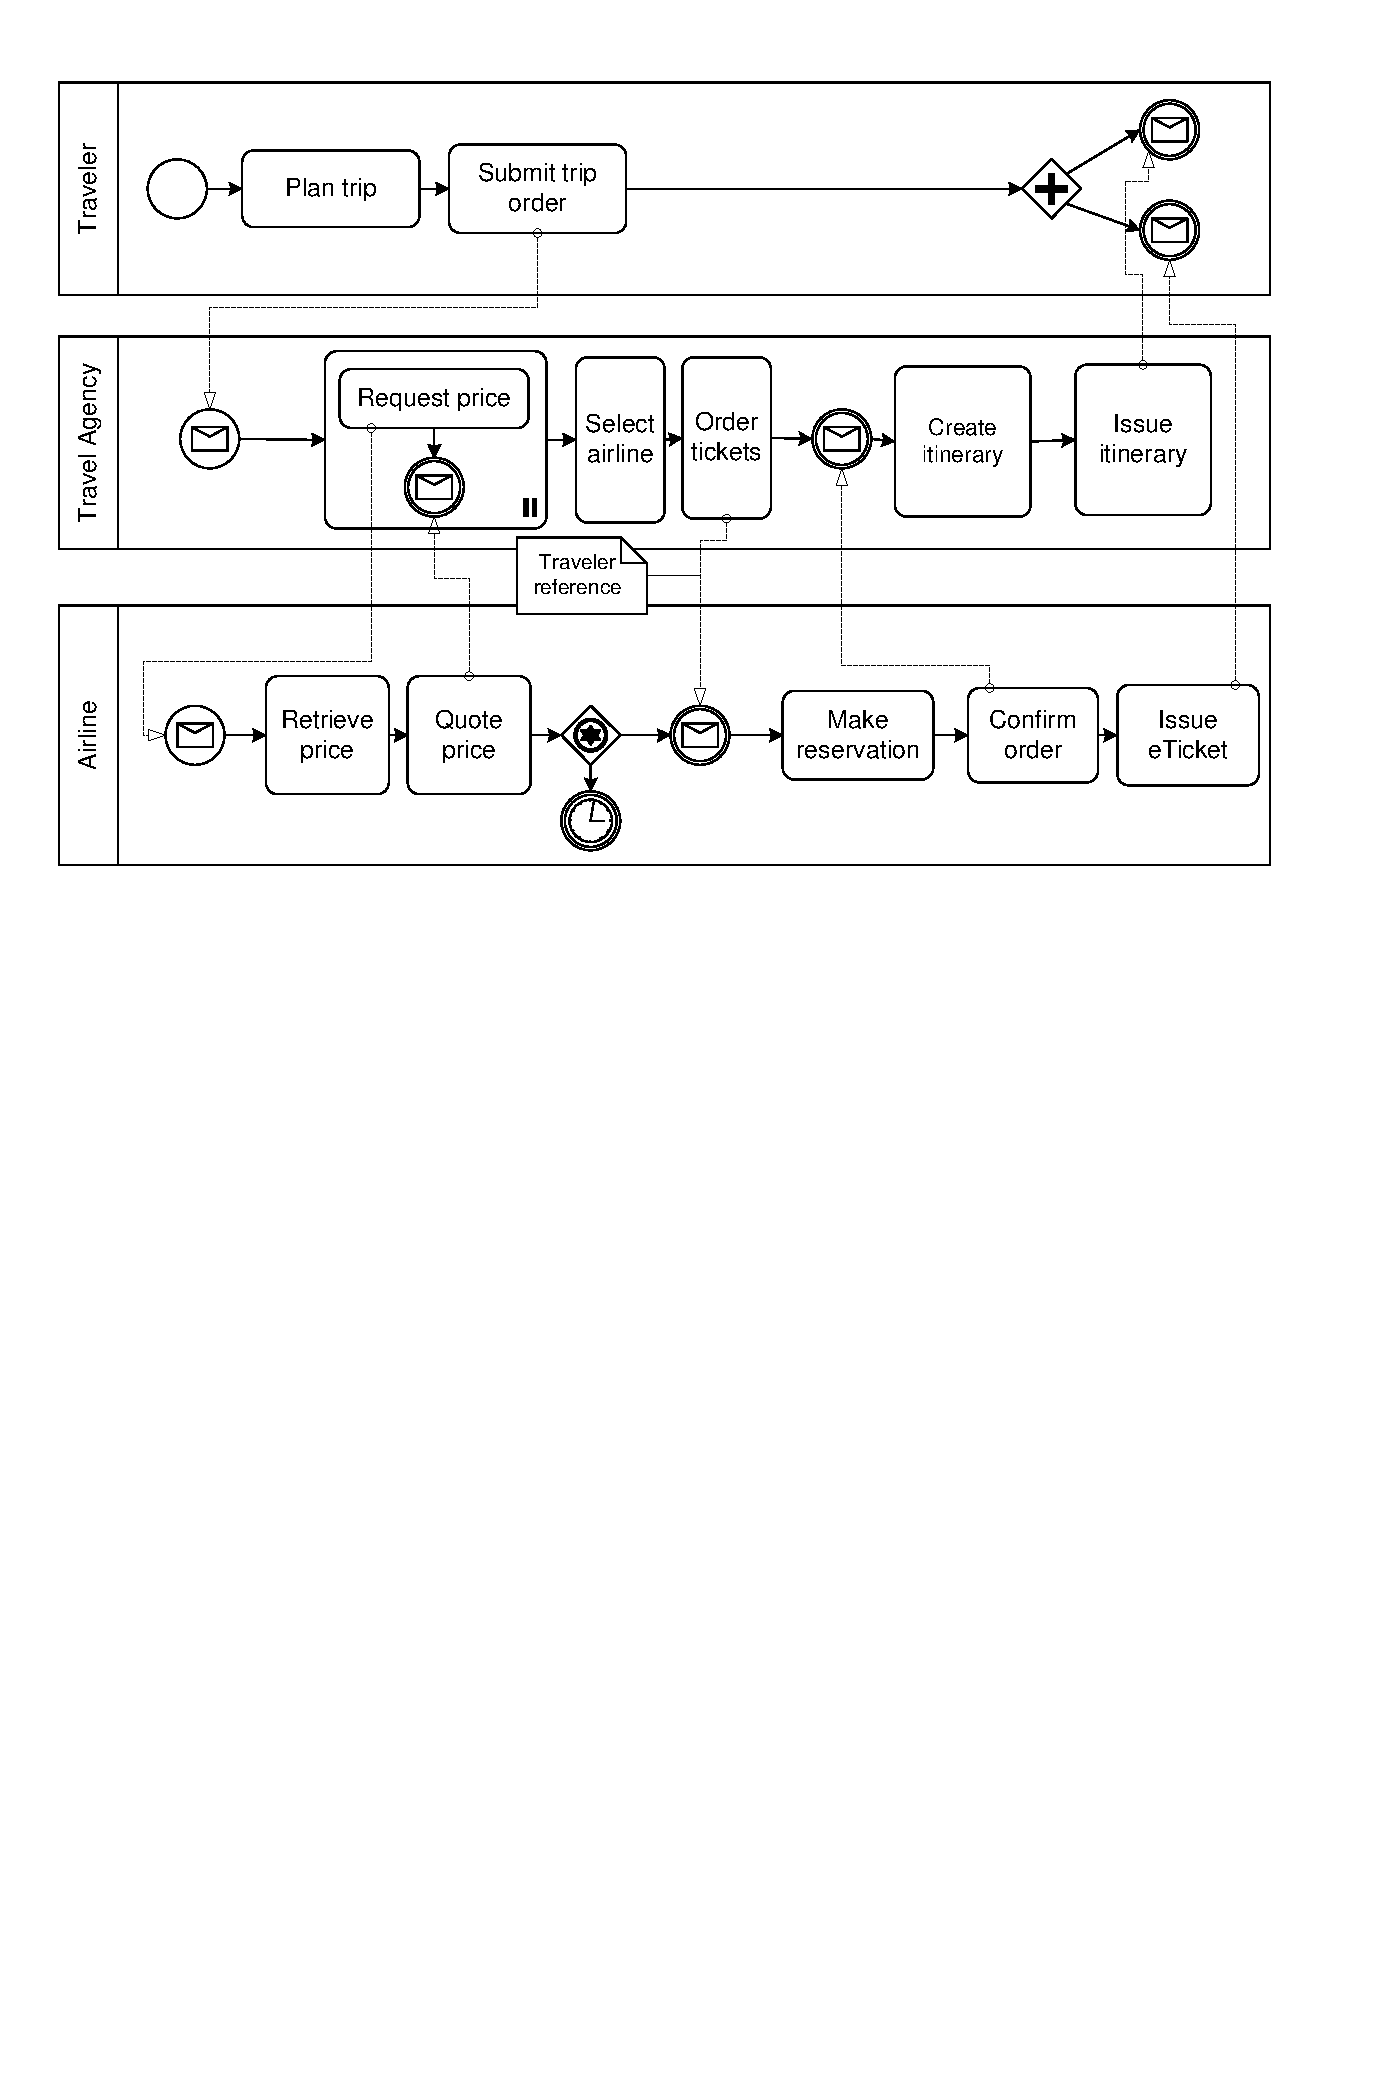
\includegraphics[width=\textwidth]{choreography.pdf}
  \caption{Beispiel-Choreographie}
  \label{fig:chor1}
\end{figure}



\begin{figure}
  \centering
  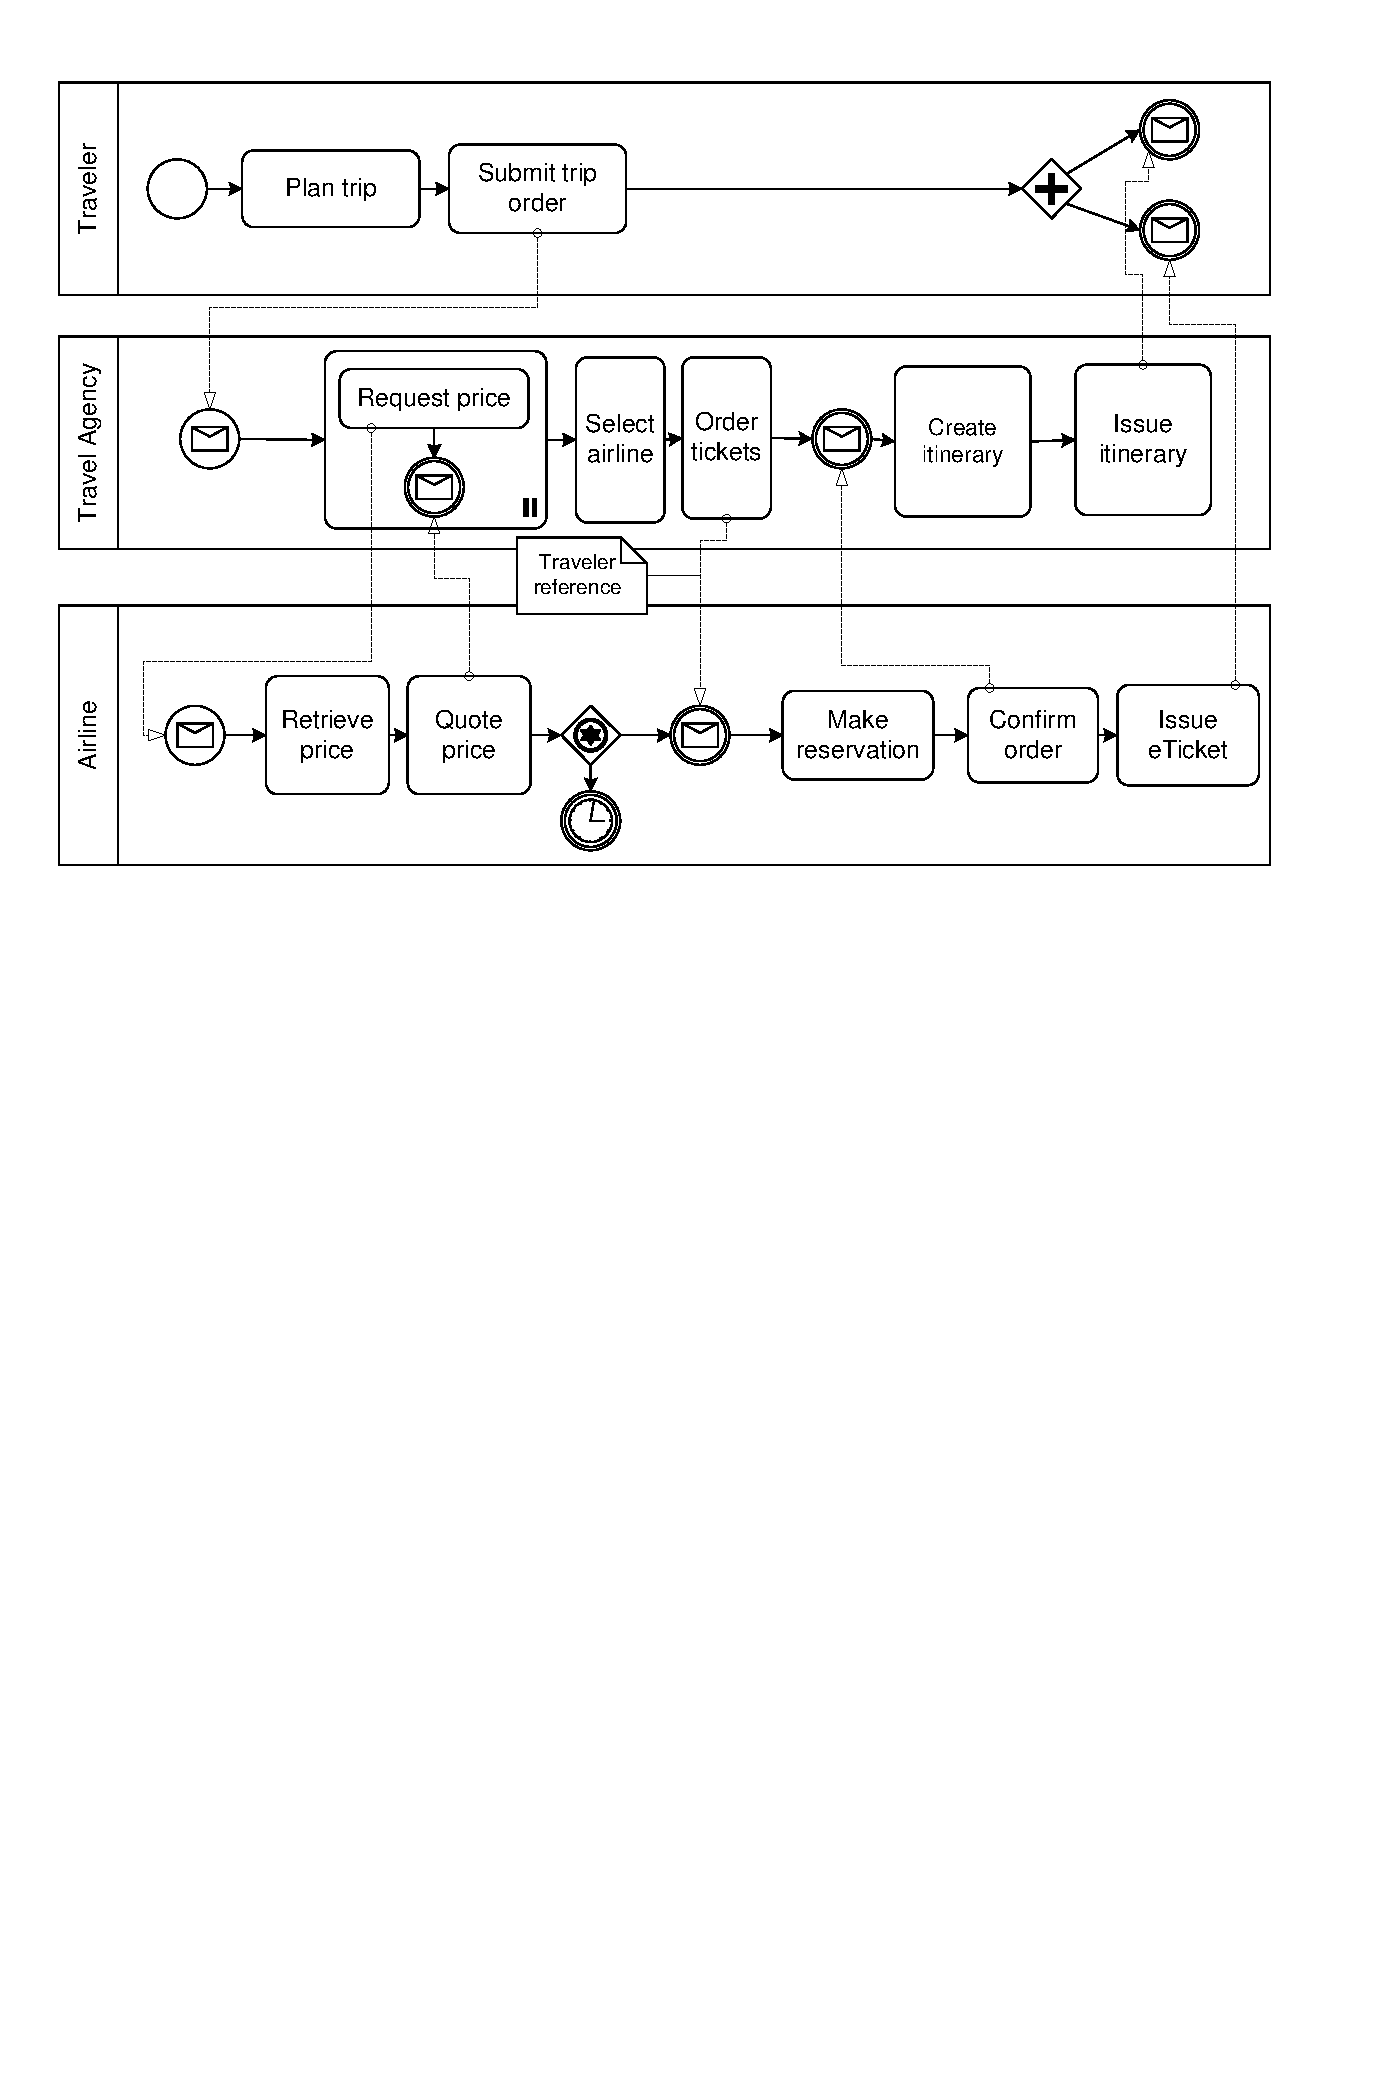
\includegraphics[width=.8\textwidth]{choreography.pdf}
  \caption[Beispiel-Choreographie]{Die Beispiel-Choreographie.
    Nun etwas kleiner, damit \texttt{\textbackslash textwidth} demonstriert wird.
    Und auch die Verwendung von alternativen Bildunterschriften für das Verzeichnis der Abbildungen.
    Letzteres ist allerdings nur Bedingt zu empfehlen, denn wer liest schon so viel Text unter einem Bild?
    Oder ist es einfach nur Stilsache?
  }
  \label{fig:chor2}
\end{figure}


\begin{figure}
  \hfill
  \begin{subfigure}{.3\textwidth}
    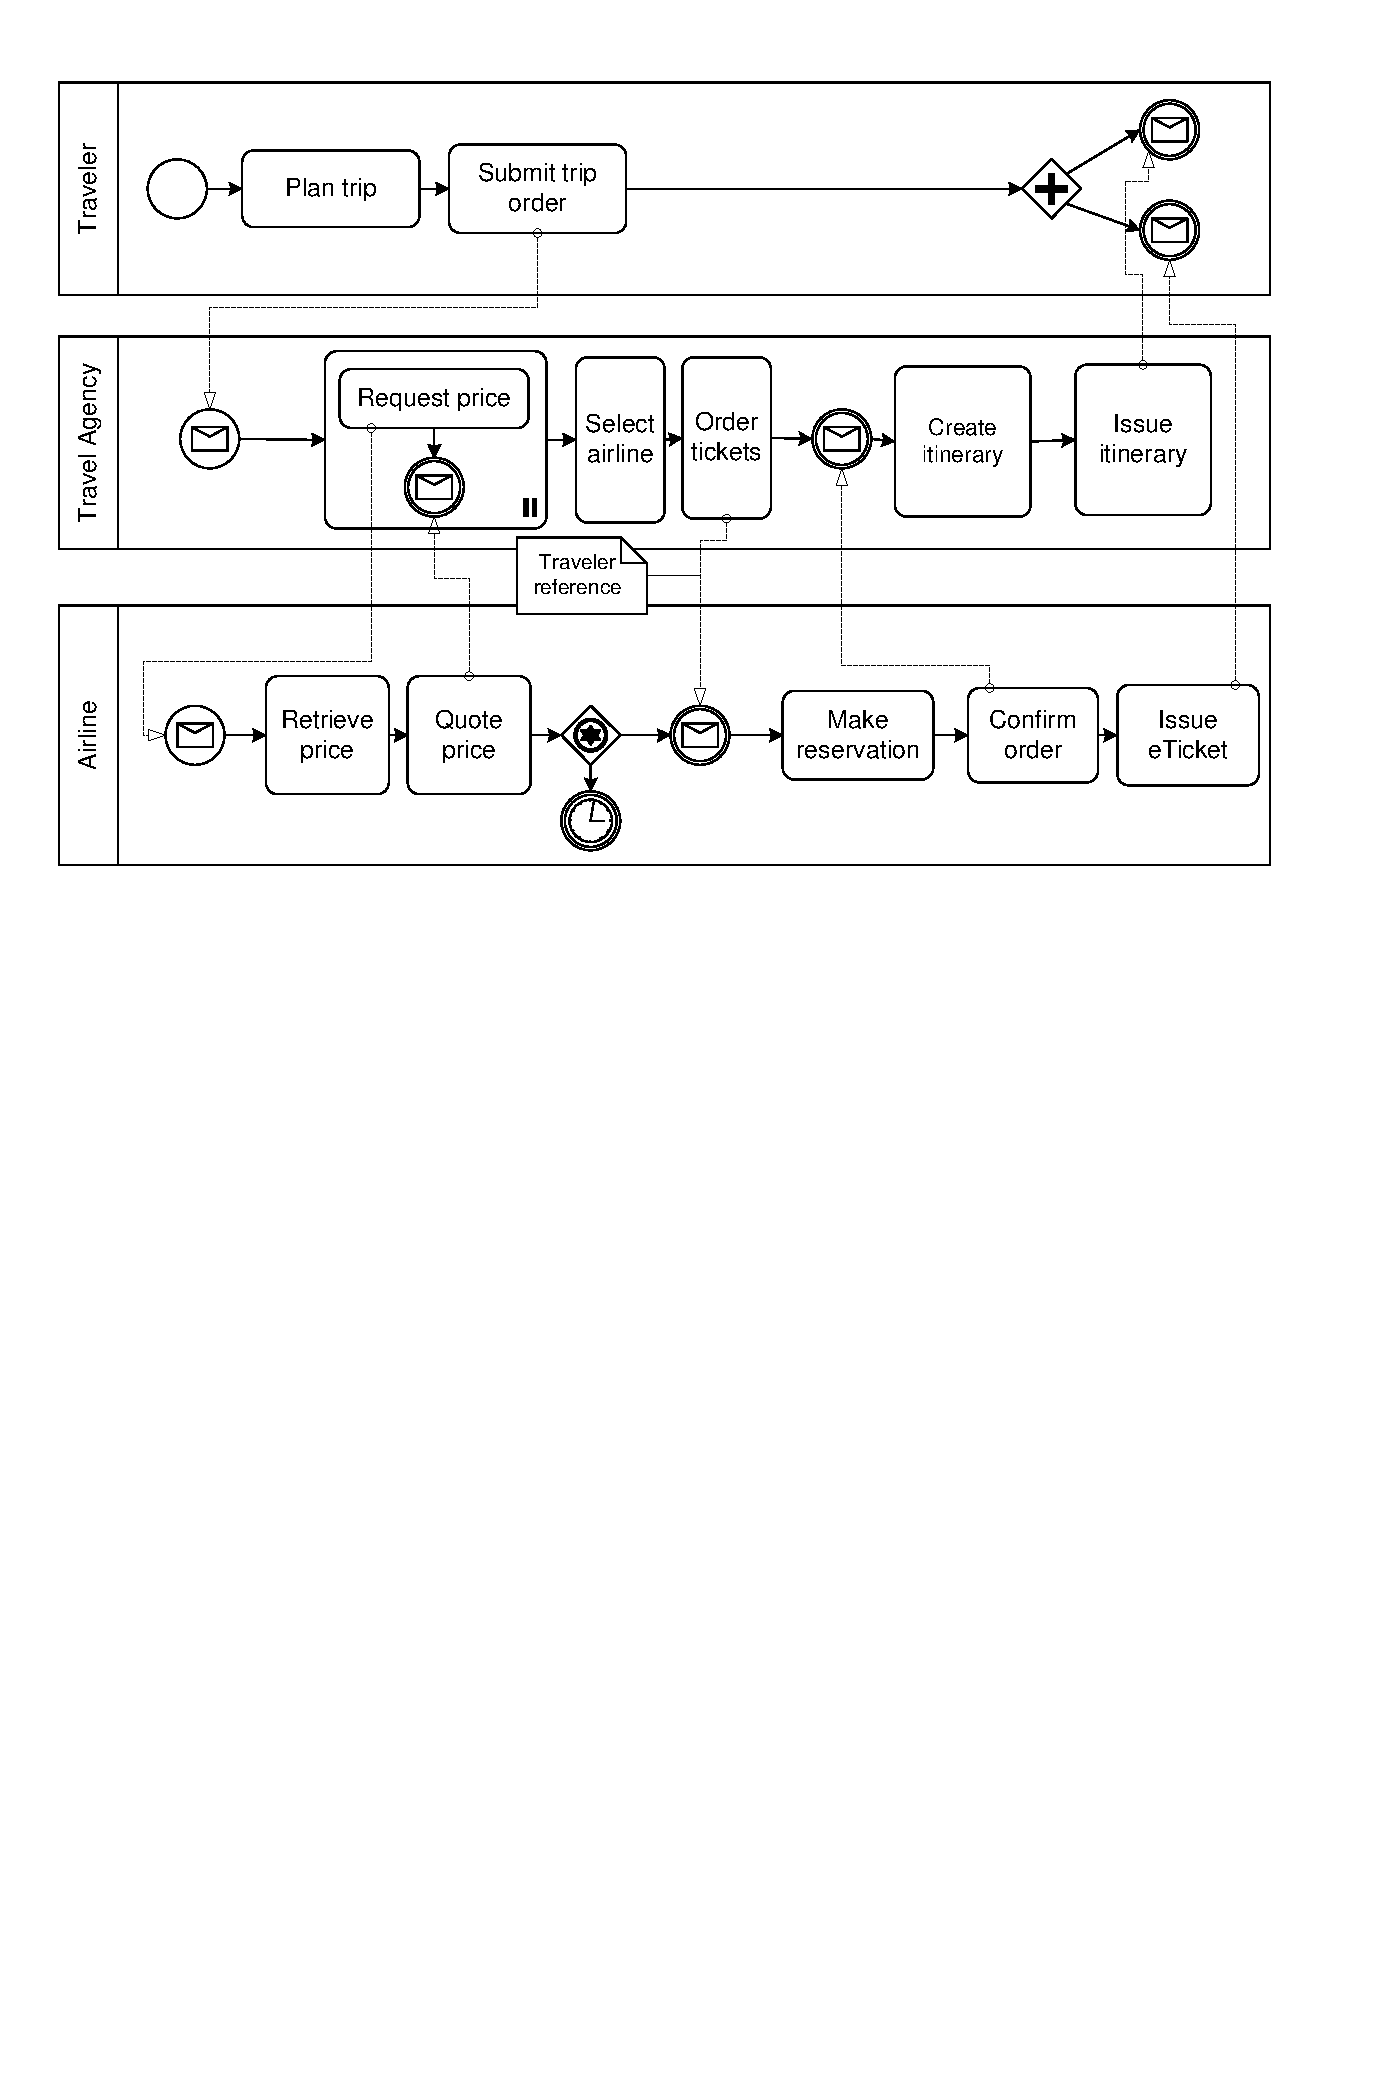
\includegraphics[width=\textwidth]{choreography.pdf}
    \caption{Choreografie 1}
    \label{fig:subfigA}
  \end{subfigure}
  \hfill
  \begin{subfigure}{.3\textwidth}
    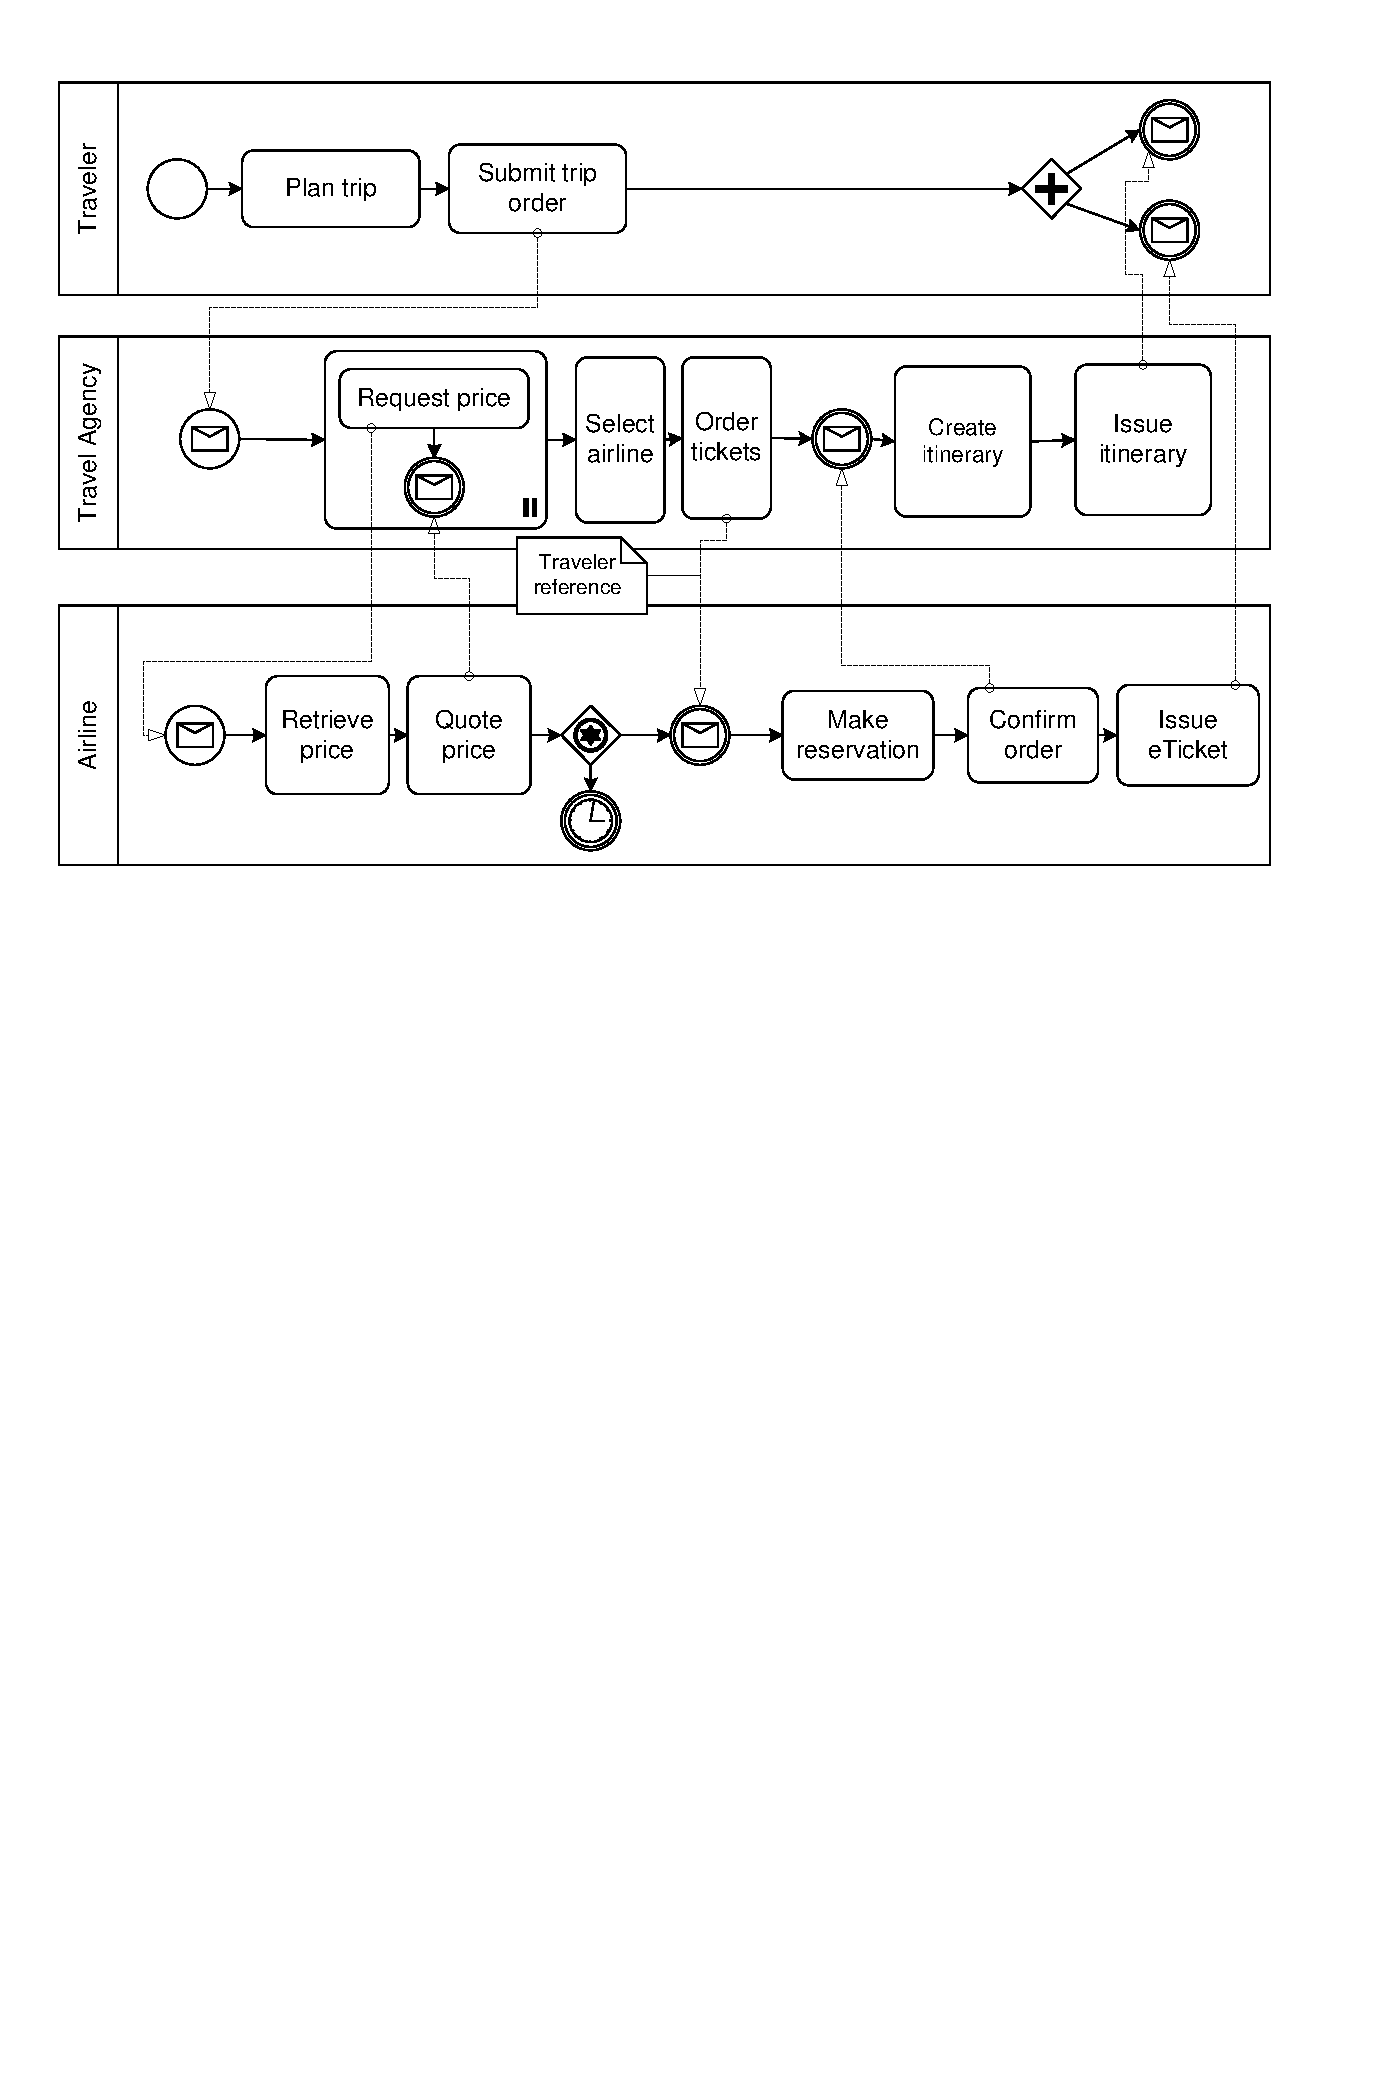
\includegraphics[width=\textwidth]{choreography.pdf}
    \caption{Choreografie 2}
    \label{fig:subfigB}
  \end{subfigure}
  \hfill
  \begin{subfigure}{.3\textwidth}
    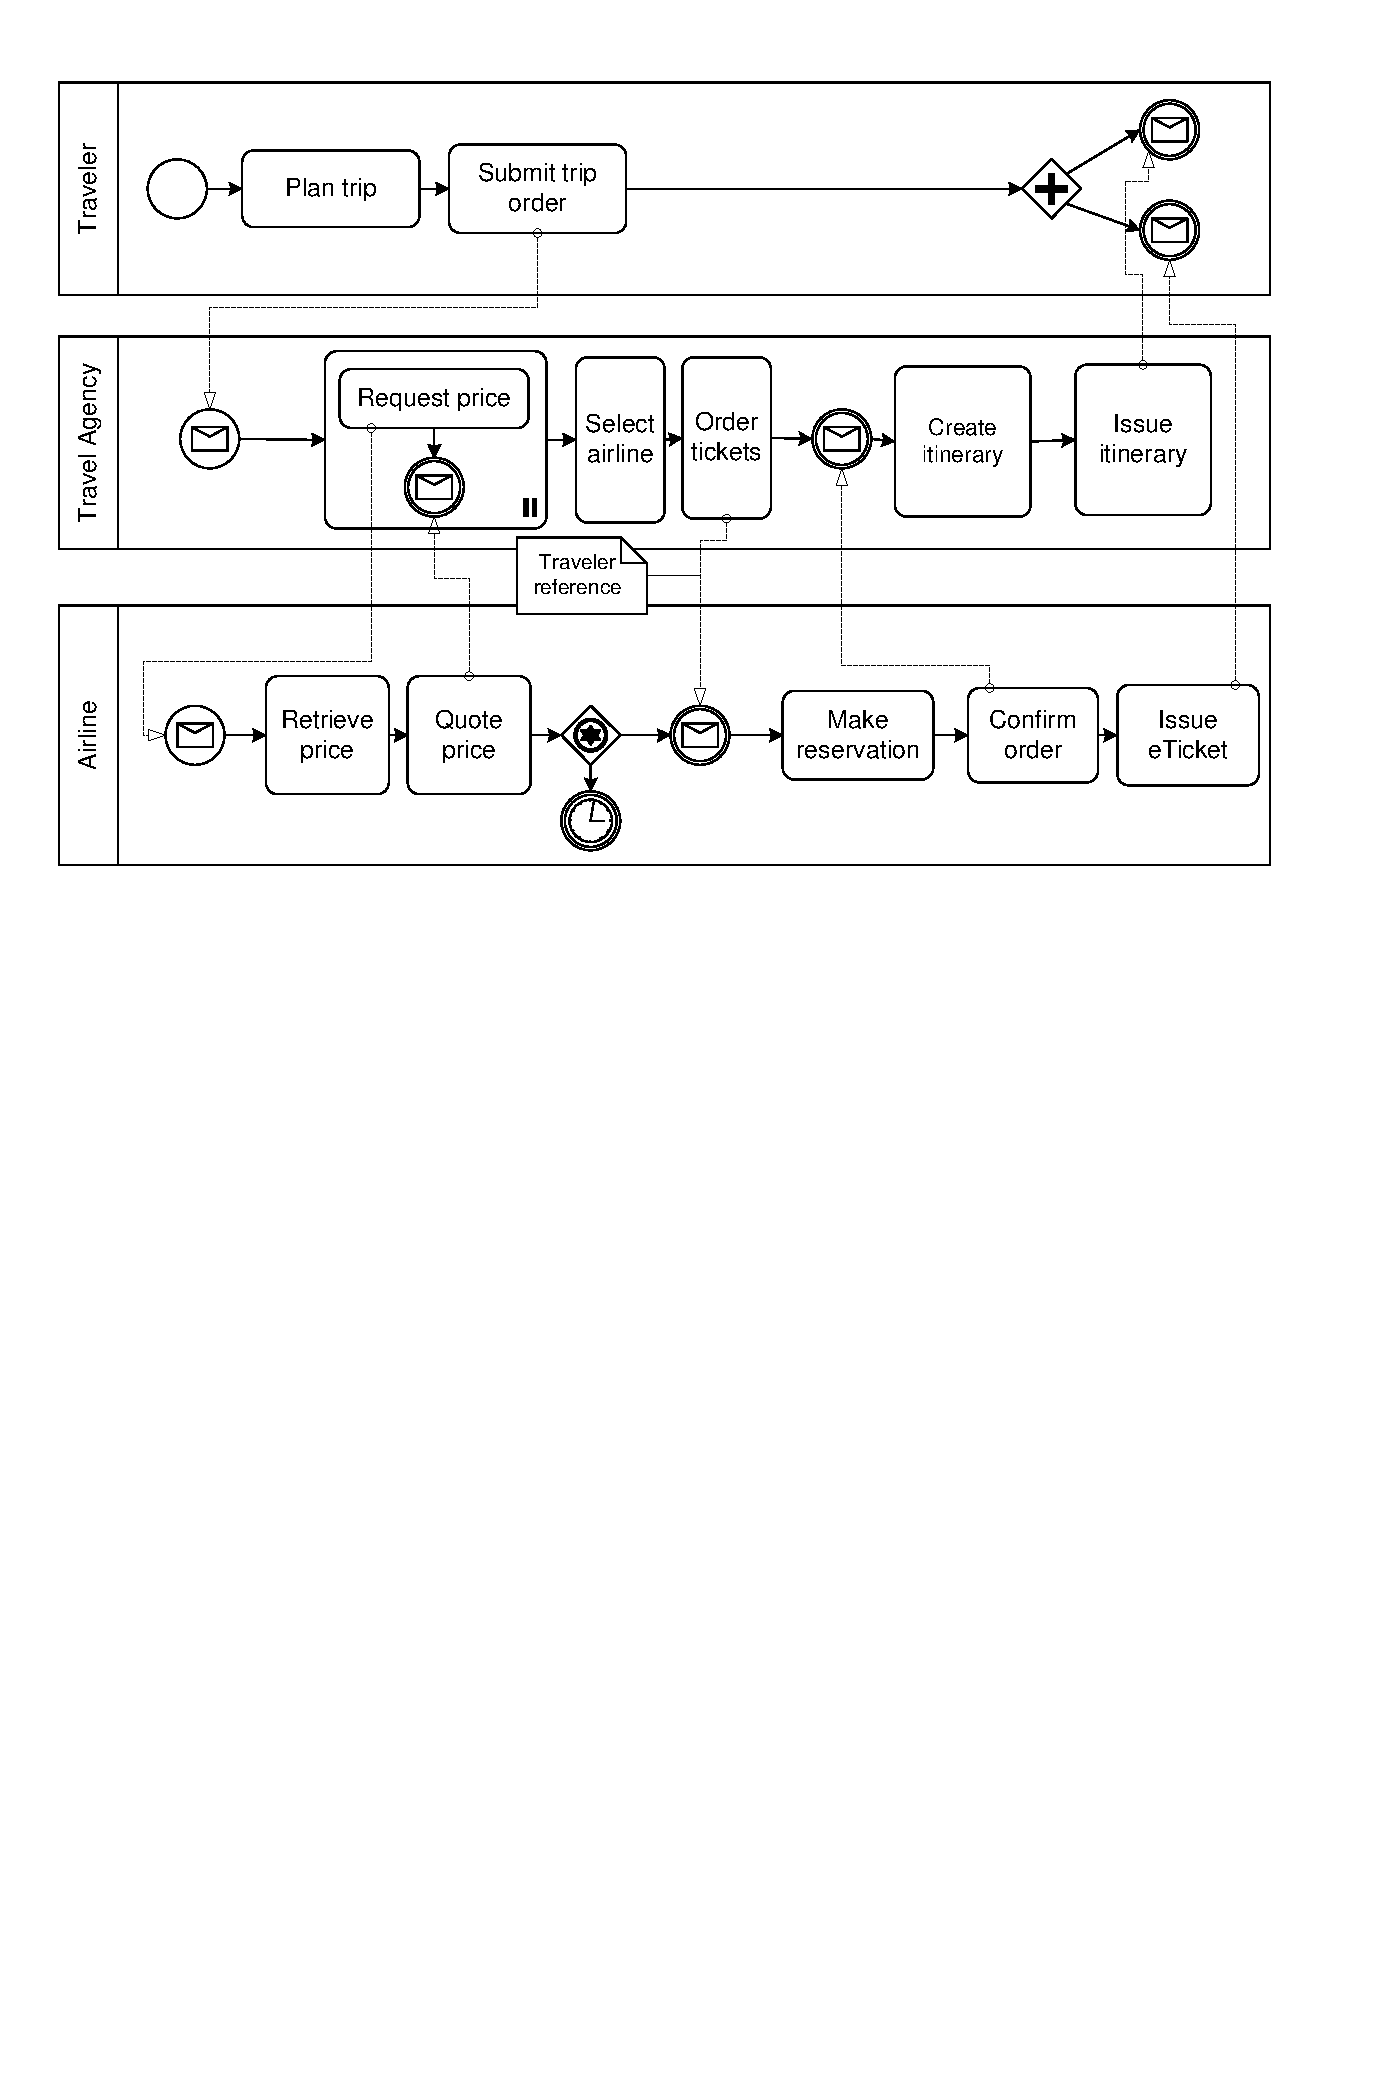
\includegraphics[width=.9\textwidth]{choreography.pdf}
    \caption{Choreografie 3}
    \label{fig:subfigC}
  \end{subfigure}
  \caption{Beispiel um 3 Abbildung nebeneinader zu stellen nur jedes einzeln referenzieren zu können.}
  \label{fig:subfig_example}
\end{figure}

\Cref{fig:subfig_example} zeigt die Verwendung des subcaption-Pakets.
Es ist auch möglich, auf Unterabbildungen zu verweisen: \Cref{fig:subfigA}.

Es ist möglich, SVGs direkt beim Kompilieren in PDF umzuwandeln.
Dies ist im Quellcode zu latex-tipps.tex beschrieben, allerdings auskommentiert.

\iffalse % <-- Das hier wegnehmen, falls inkscape im Pfad ist
  Das SVG in \cref{fig:directSVG} ist direkt eingebunden, während der Text im SVG in \cref{fig:latexSVG} mittels pdflatex gesetzt ist.
  Falls man die Graphiken sehen möchte, muss inkscape im PATH sein und im Tex-Quelltext \texttt{\textbackslash{}iffalse} und \texttt{\textbackslash{}iftrue} auskommentiert sein.

  \begin{figure}
    \centering
    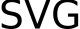
\includegraphics{svgexample.svg}
    \caption{SVG direkt eingebunden}
    \label{fig:directSVG}
  \end{figure}

  \begin{figure}
    \centering
    \def\svgwidth{.4\textwidth}
    \includesvg{svgexample}
    \caption{Text im SVG mittels \LaTeX{} gesetzt}
    \label{fig:latexSVG}
  \end{figure}
\fi % <-- Das hier wegnehmen, falls inkscape im Pfad ist


\section{Weitere Illustrationen}
\Cref{fig:AnhangsChor,fig:AnhangsChor2} zeigen zwei Choreographien, die den Sachverhalt weiter erläutern sollen.
Die zweite Abbildung ist um 90 Grad gedreht, um das Paket \texttt{pdflscape} zu demonstrieren.

\begin{figure}
  \centering
  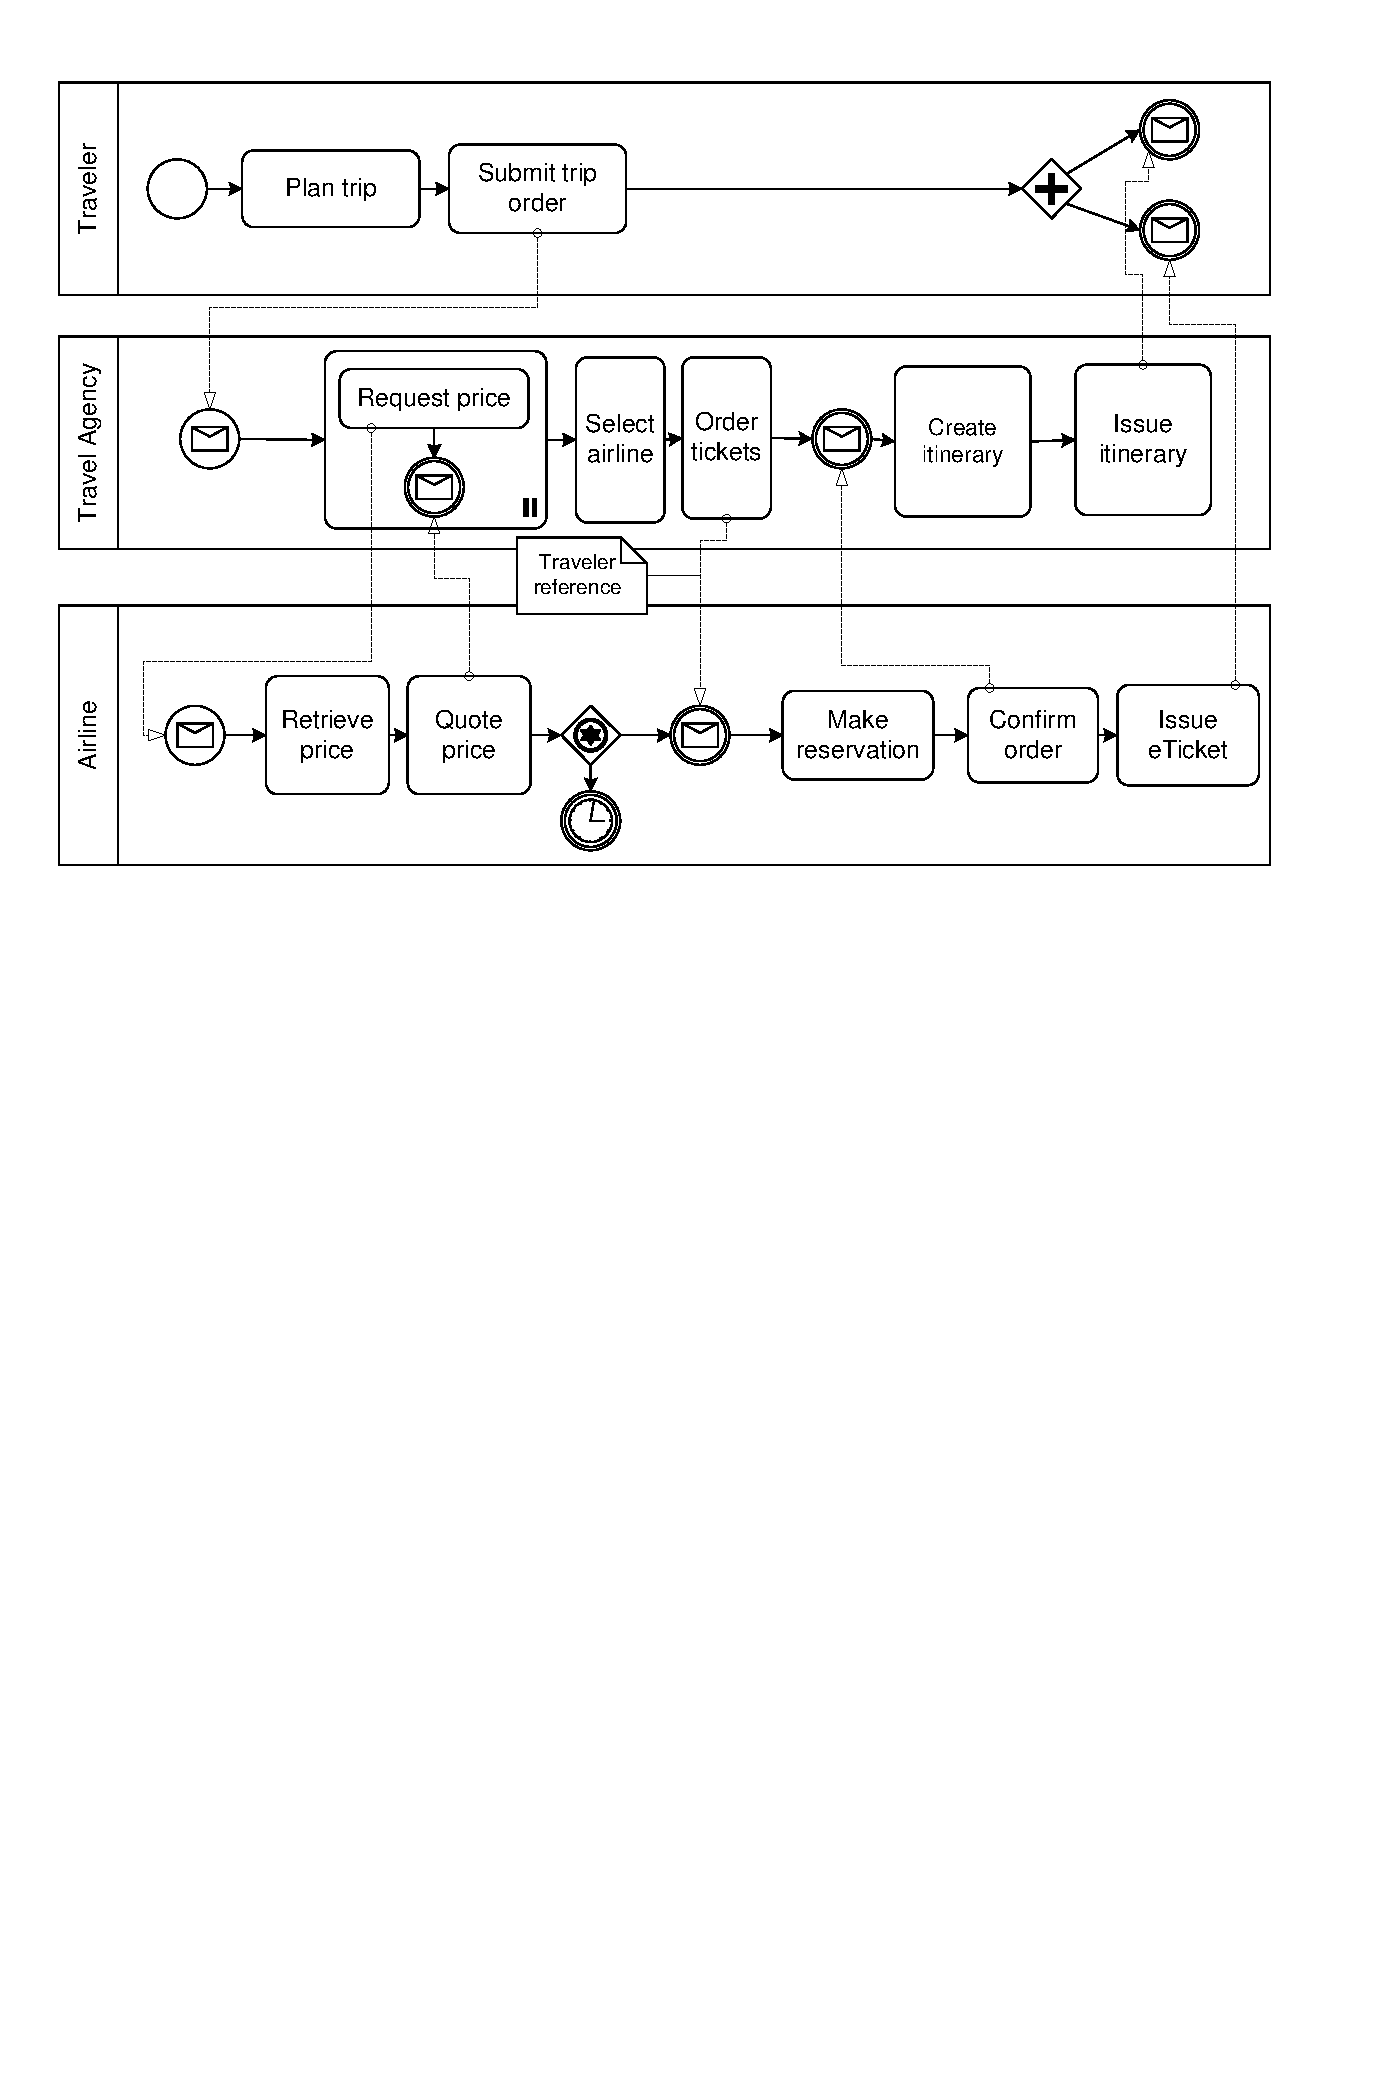
\includegraphics[width=\textwidth]{choreography.pdf}
  \caption{Beispiel-Choreographie I}
  \label{fig:AnhangsChor}
\end{figure}

\begin{landscape}
  \begin{figure}
    \centering
    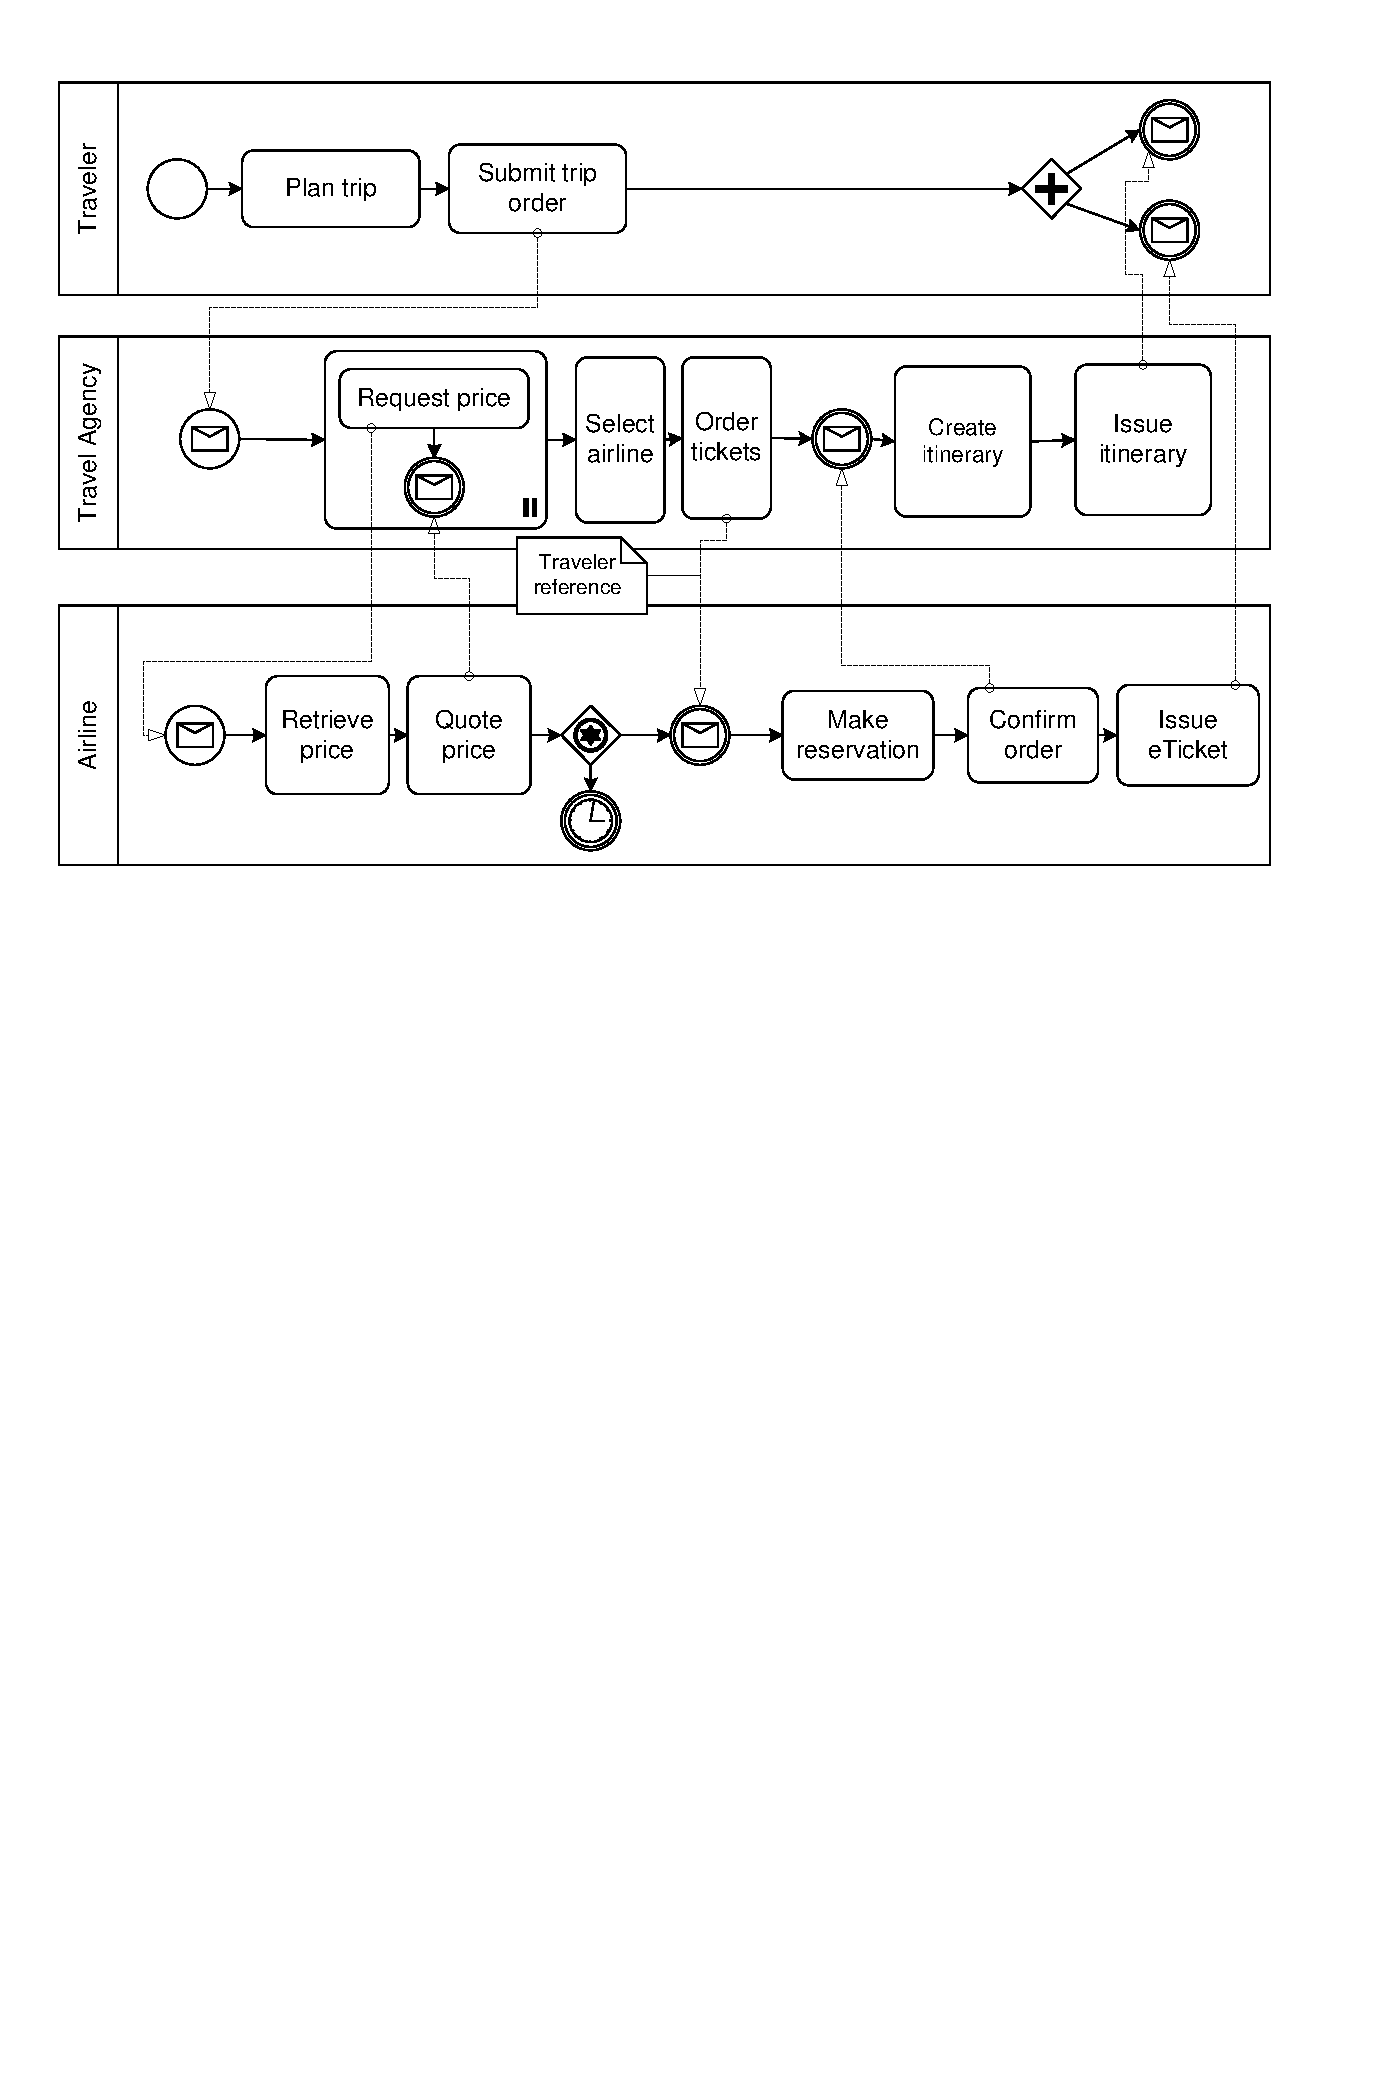
\includegraphics[width=\textwidth]{choreography.pdf}
    \caption{Beispiel-Choreographie II}
    \label{fig:AnhangsChor2}
  \end{figure}
\end{landscape}


\iffalse

  \clearpage

  FIXME - This does not work with MiKTeX as of 2016-12-30

  TODO- demonstrate rotating package

  %hint by http://tex.stackexchange.com/a/3265/9075
  %other option is to use changepage according to http://tex.stackexchange.com/a/2639/9075. This, however, has issues with landscape
  \thispagestyle{empty}

  \savegeometry{koma}

  %If you only have height problems, this is not needed at all
  \addtolength{\textwidth}{2cm}
  \addtolength{\evensidemargin}{-1cm}

  \begin{landscape}
    %sidewaysfigure
    \begin{figure}
      \centering
      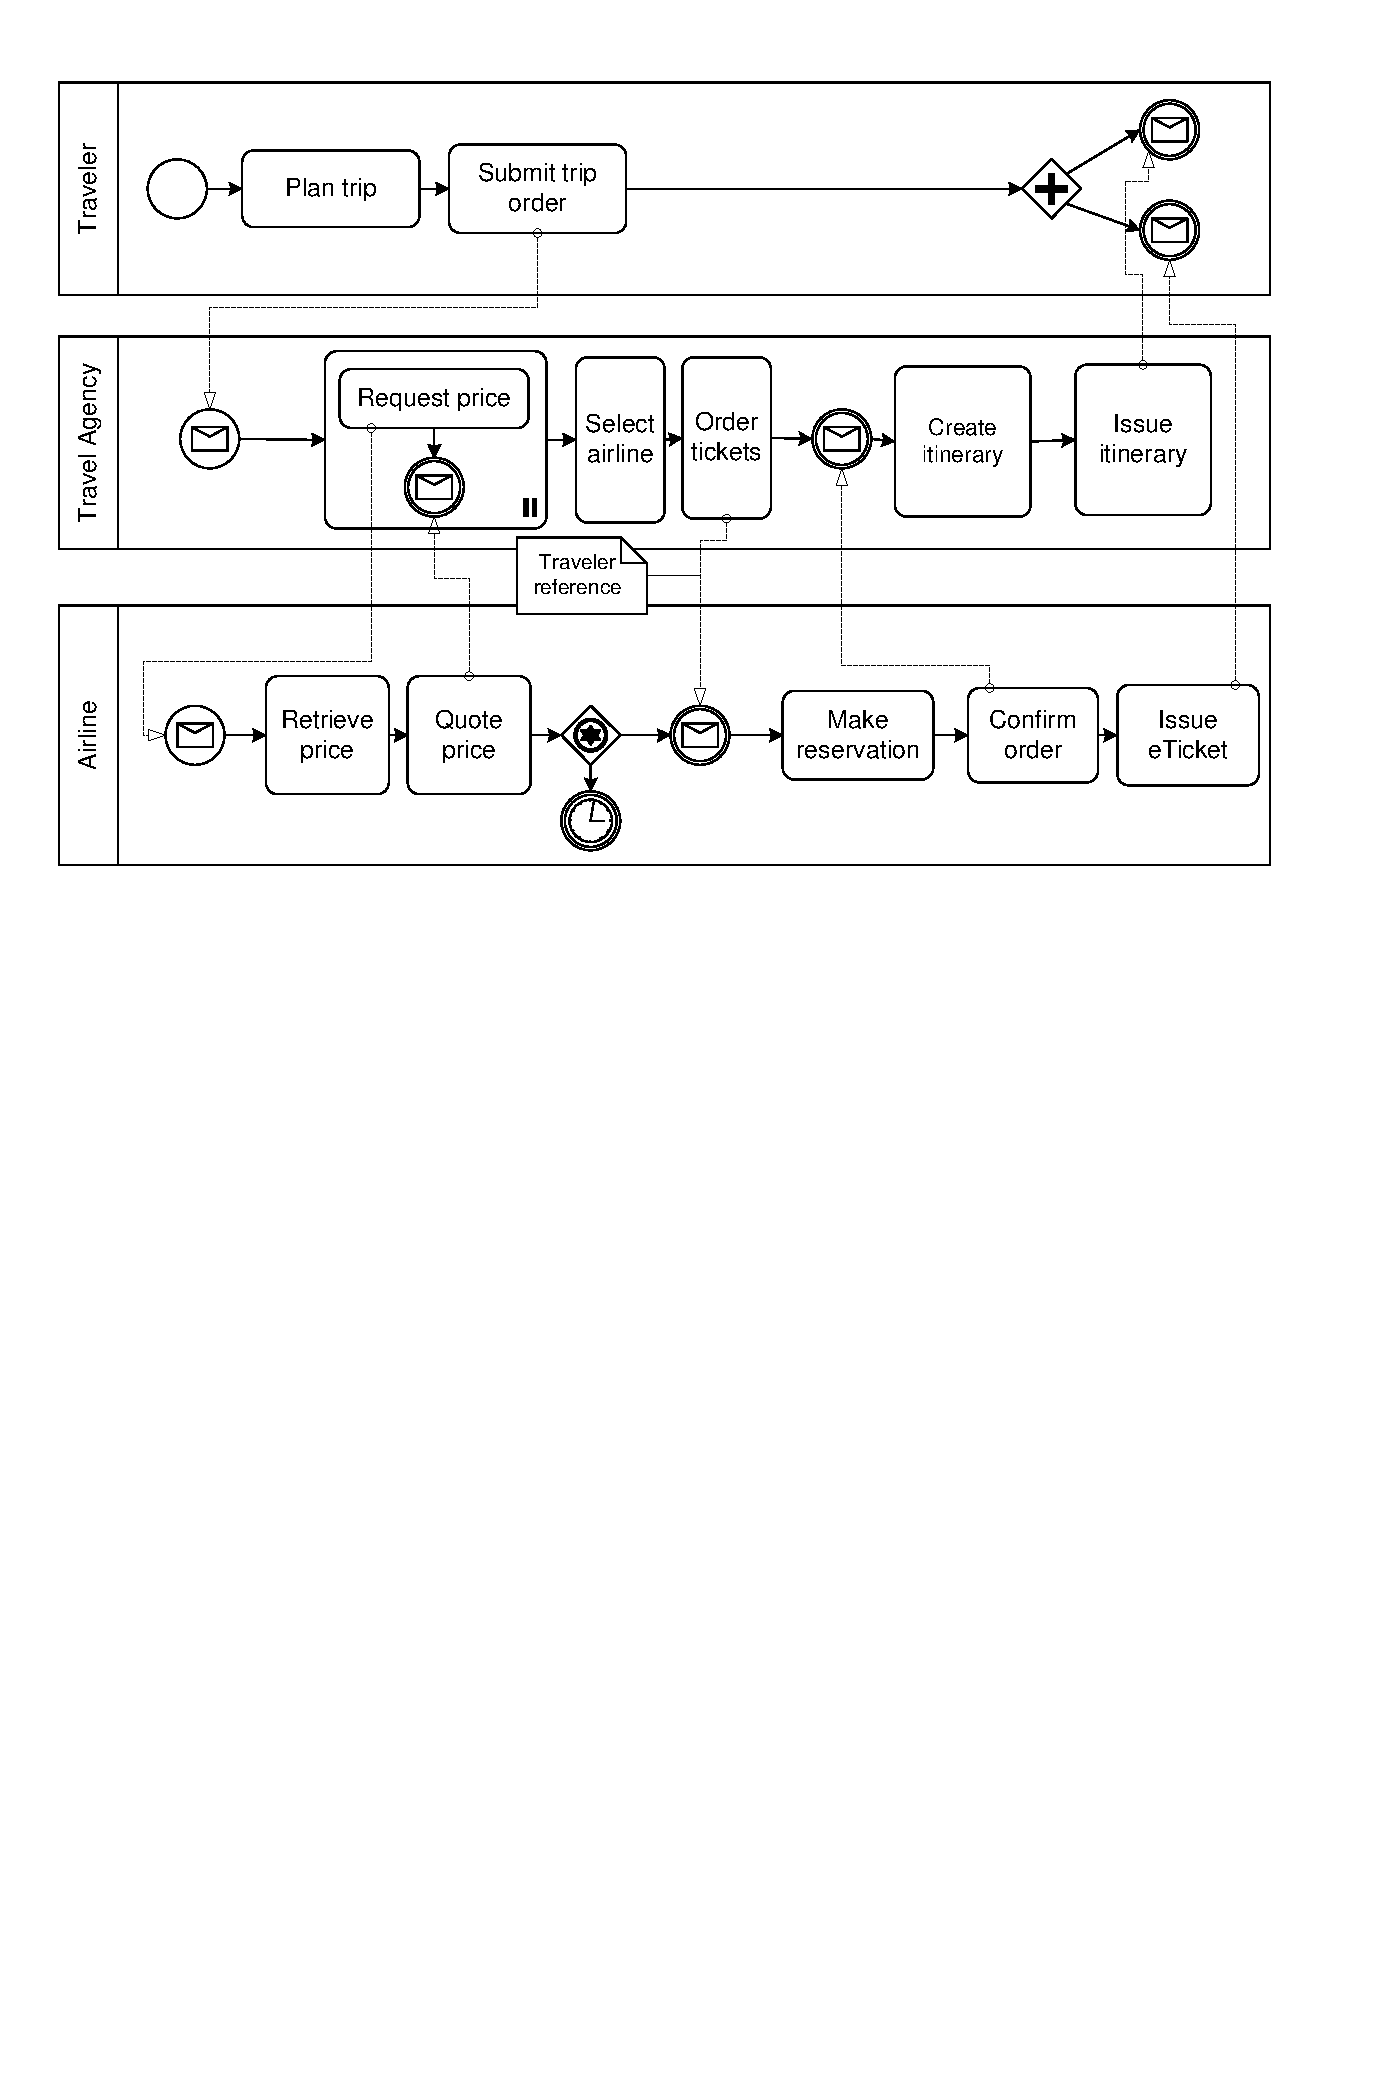
\includegraphics[width=0.9\paperheight]{choreography.pdf}
      \caption{Beispiel-Choreographie, auf einer weißen Seite gezeigt wird und über die definierten Seitenränder herausragt}
    \end{figure}
  \end{landscape}

  %the original layout is restored.
  %%\restoregeometry cannot be used as we use \addtolength
  \loadgeometry{koma}

\fi

\IfFileExists{pgfplots.sty}{
  \section{Plots with pgfplots}
  Pgfplot ist ein Paket um Graphen zu plotten ohne den Umweg über gnuplot oder matplotlib zu gehen.
  %hint by http://tex.stackexchange.com/a/3265/9075%other option is to use changepage according to http://tex.stackexchange.com/a/2639/9075. This, however, has issues with landscape%If you only have height problems, this is not needed at all%sidewaysfigure%the original layout is restored.%%\restoregeometry cannot be used as we use \addtolength
  \begin{figure}[h]
    \begin{center}
      \begin{tikzpicture}
        \begin{axis}[xlabel=$x$,
            ylabel=$\sin(x)$]
          \addplot {sin(deg(x))};  % Sinus-Funktion zeichnen
        \end{axis}
      \end{tikzpicture}
    \end{center}
    \caption{$\sin(x)$ mit pgfplots.}
  \end{figure}

   \begin{figure}[h]
    \begin{center}
      \begin{tikzpicture}
        \begin{axis}[xlabel=$x$,
            ylabel=$y$]
          \addplot table [x=a, y=c, col sep=comma] {data/data.csv};  % Koordinaten aus einer CSV-Datei lesen und plotten
        \end{axis}
      \end{tikzpicture}
    \end{center}
    \caption{Koordianten $x$ und $y$ aus einer CSV-Datei geplottet mit pgfplots.}
  \end{figure}

}{}

\section{Figures with tikz}
TikZ ist ein Paket um Zeichnungen mittels Programmierung zu erstellen.
Dieses Paket eignet sich um Gitter zu erstellen oder andere regelmäßige Strukturen zu erstellen.
Hier gibt es sehr viele visuelle Beispiele was tikz alles kann\footnote{\url{http://texdoc.net/pkg/visualtikz}}.

\begin{figure}[ht]
  \begin{center}
    \begin{tikzpicture}
      \draw(0,0) rectangle (4,4);
      \foreach \x in {0.5,1,1.5,2,2.5,3,3.5}
      \foreach \y in {0.5,1,1.5,2,2.5,3,3.5}
      \draw(\x,\y) circle (1pt);
    \end{tikzpicture}
  \end{center}
  \caption{Eine tikz-Graphik.}\label{fig:tikz_example}
\end{figure}


\section{UML-Diagramme mit tikz-uml}

\Cref{fig:uml} zeigt ein Klassendiagramm, das mittels tikz-uml gesetzt wurde.

\begin{center}
\begin{figure}
\begin{tikzpicture}
\begin{umlpackage}{p}
\begin{umlpackage}{sp1}
\umlclass[template=T]{A}{
  n : uint \\ t : float
}{}
\umlclass[y=-3]{B}{
  d : double
}{
  \umlvirt{setB(b : B) : void} \\ getB() : B}
\end{umlpackage}
\begin{umlpackage}[x=10,y=-6]{sp2}
\umlinterface{C}{
  n : uint \\ s : string
}{}
\end{umlpackage}
\umlclass[x=2,y=-10]{D}{
  n : uint
  }{}
\end{umlpackage}

\umlassoc[geometry=-|-, arg1=tata, mult1=*, pos1=0.3, arg2=toto, mult2=1, pos2=2.9, align2=left]{C}{B}
\umlunicompo[geometry=-|, arg=titi, mult=*, pos=1.7, stereo=vector]{D}{C}
\umlimport[geometry=|-, anchors=90 and 50, name=import]{sp2}{sp1}
\umlaggreg[arg=tutu, mult=1, pos=0.8, angle1=30, angle2=60, loopsize=2cm]{D}{D}
\umlinherit[geometry=-|]{D}{B}
\umlnote[x=2.5,y=-6, width=3cm]{B}{Eine Notiz f\"ur die Klasse B}
\umlnote[x=7.5,y=-2]{import-2}{Eine Anmerkung}
\end{tikzpicture}
\caption{Ein Klassendiagramm mit tikz-uml generiert. Beispiel von Nicolas Kielbasiewicz adaptiert.}
\label{fig:uml}
\end{figure}
\end{center}

\section{Tabellen}

\cref{tab:Ergebnisse} zeigt Ergebnisse und die \cref{tab:Ergebnisse} zeigt wie numerische Daten in einer Tabelle representiert werden können.
\begin{table}
  \centering
  \begin{tabular}{ccc}
    \toprule
    \multicolumn{2}{c}{\textbf{zusammengefasst}} & \textbf{Titel}                                                          \\ \midrule
    Tabelle                                      & wie                                                           & in      \\
    \url{tabsatz.pdf}                            & empfohlen                                                     & gesetzt \\

    \multirow{2}{*}{Beispiel}                    & \multicolumn{2}{c}{ein schönes Beispiel}                                \\
                                                 & \multicolumn{2}{c}{für die Verwendung von \qq{multirow}}           \\
    \bottomrule
  \end{tabular}
  \caption[Beispieltabelle]{Beispieltabelle -- siehe \url{http://www.ctan.org/tex-archive/info/german/tabsatz/}}
  \label{tab:Ergebnisse}
\end{table}

\begin{table}
  \centering
  \begin{tabular}{l *{8}{d{3.2}}}
    \toprule

                         & \multicolumn{2}{c}{\textbf{Parameter 1}} & \multicolumn{2}{c}{\textbf{Parameter 2}} & \multicolumn{2}{c}{\textbf{Parameter 3}} & \multicolumn{2}{c}{\textbf{Parameter 4}}                                                                                                                                       \\
    \cmidrule(r){2-3}\cmidrule(lr){4-5}\cmidrule(lr){6-7}\cmidrule(l){8-9}

    \textbf{Bedingungen} & \multicolumn{1}{c}{\textbf{M}}           & \multicolumn{1}{c}{\textbf{SD}}          & \multicolumn{1}{c}{\textbf{M}}           & \multicolumn{1}{c}{\textbf{SD}}          & \multicolumn{1}{c}{\textbf{M}} & \multicolumn{1}{c}{\textbf{SD}} & \multicolumn{1}{c}{\textbf{M}} & \multicolumn{1}{c}{\textbf{SD}} \\
    \midrule

    W                    & 1.1                                      & 5.55                                     & 6.66                                     & .01                                      &                                &                                 &                                &                                 \\
    X                    & 22.22                                    & 0.0                                      & 77.5                                     & .1                                       &                                &                                 &                                &                                 \\
    Y                    & 333.3                                    & .1                                       & 11.11                                    & .05                                      &                                &                                 &                                &                                 \\
    Z                    & 4444.44                                  & 77.77                                    & 14.06                                    & .3                                       &                                &                                 &                                &                                 \\
    \bottomrule
  \end{tabular}

  \caption{
    Beispieltabelle f\"{u}r 4 Bedingungen (W-Z) mit jeweils 4 Parameters mit (M und SD).
    Hinweis: Stets die selbe Anzahl an Nachkommastellen angeben.
  }
  \label{tab:Werte}
\end{table}



\IfFileExists{pgfplotstable.sty}{

\subsection{Tabellen mit pgfplots}
Mit pgfplots koennen Tabellen direkt aus einer CSV-Datei erstellt werden.

\begin{table}[h]
\centering
\pgfplotstabletypeset[
col sep = comma,
every head row/.style={before row=\toprule,after row=\midrule},
every last row/.style={after row=\bottomrule},
display columns/0/.style={string type,column name={}}
]
{data/data.csv}
\caption{Tabelle generiert aus einer CSV-Datei mit pgfplots}
\end{table}
}{}


\section{Tabellen über mehere Seiten}

\begin{longtable}{|l|l|l|}
\caption{Tabelle \"uber mehere Seiten} \label{tab:long} \\

\hline \multicolumn{1}{|c|}{\textbf{A}} & \multicolumn{1}{c|}{\textbf{B}} & \multicolumn{1}{c|}{\textbf{B}} \\ \hline
\endfirsthead

\multicolumn{3}{c}%
{{\bfseries \tablename\ \thetable{} -- von dor vorherigen Seite weitergeführt}} \\
\hline \multicolumn{1}{|c|}{\textbf{First column}} & \multicolumn{1}{c|}{\textbf{Second column}} & \multicolumn{1}{c|}{\textbf{Third column}} \\ \hline
\endhead

\hline \multicolumn{3}{|r|}{{Wird auf der n\"achsten Seite fortgef\"uhrt}} \\ \hline
\endfoot

\hline \hline
\endlastfoot

A & B C & D \\
A & B C & D \\
A & B C & D \\
A & B C & D \\
A & B C & D \\
A & B C & D \\
A & B C & D \\
A & B C & D \\
A & B C & D \\
A & B C & D \\
A & B C & D \\
A & B C & D \\
A & B C & D \\
A & B C & D \\
A & B C & D \\
A & B C & D \\
A & B C & D \\
A & B C & D \\
A & B C & D \\
A & B C & D \\
A & B C & D \\
A & B C & D \\
A & B C & D \\
A & B C & D \\
A & B C & D \\
A & B C & D \\
A & B C & D \\
A & B C & D \\
A & B C & D \\
A & B C & D \\
A & B C & D \\
A & B C & D \\
A & B C & D \\
A & B C & D \\
A & B C & D \\
A & B C & D \\
A & B C & D \\
A & B C & D \\
A & B C & D \\
A & B C & D \\
A & B C & D \\
A & B C & D \\
A & B C & D \\
A & B C & D \\
A & B C & D \\
A & B C & D \\
A & B C & D \\
A & B C & D \\
A & B C & D \\
A & B C & D \\
A & B C & D \\
A & B C & D \\
A & B C & D \\
A & B C & D \\
A & B C & D \\
A & B C & D \\
A & B C & D \\
A & B C & D \\
A & B C & D \\
A & B C & D \\
A & B C & D \\
A & B C & D \\
A & B C & D \\
A & B C & D \\
A & B C & D \\
A & B C & D \\
A & B C & D \\
A & B C & D \\
A & B C & D \\
A & B C & D \\
A & B C & D \\
A & B C & D \\
A & B C & D \\
A & B C & D \\
A & B C & D \\
A & B C & D \\
A & B C & D \\
A & B C & D \\
A & B C & D \\
A & B C & D \\
\end{longtable}


\section{Abkürzungen}

Beim ersten Durchlauf betrug die \gls{fr} 5.
Beim zweiten Durchlauf war die \gls{fr} 3.
Die Pluralform sieht man hier: \glspl{er}.
Um zu demonstrieren, wie das Abkürzungsverzeichnis bei längeren Beschreibungstexten aussieht, muss hier noch \glspl{rdbms} erwähnt werden.

Mit \verb+\gls{...}+ können Abkürzungen eingebaut werden, beim ersten Aufrufen wird die lange Form eingesetzt.
Beim wiederholten Verwenden von \verb+\gls{...}+ wird automatisch die kurz Form angezeigt.
Außerdem wird die Abkürzung automatisch in die Abkürzungsliste eingefügt.
Mit \verb+\glspl{...}+ wird die Pluralform verwendet.
Möchte man, dass bei der ersten Verwendung direkt die Kurzform erscheint, so kann man mit \verb+\glsunset{...}+ eine Abkürzung als bereits verwendet markieren.
Das Gegenteil erreicht man mit \verb+\glsreset{...}+.

Definiert werden Abkürzungen in der Datei \textit{content\\ausarbeitung.tex} mithilfe von \verb+\newacronym{...}{...}{...}+.

Mehr Infos unter: \url{http://tug.ctan.org/macros/latex/contrib/glossaries/glossariesbegin.pdf}


\section{Verweise}
Für weit entfernte Abschnitte ist \qq{varioref} zu empfehlen:
\qq{Siehe \vref{sec:mf}}.
Das Kommando \texttt{\textbackslash{}vref} funktioniert ähnlich wie \texttt{\textbackslash{}cref} mit dem Unterschied, dass zusätzlich ein Verweis auf die Seite hinzugefügt wird.
\texttt{vref}: \qq{\vref{sec:firstsectioninlatexhints}}, \texttt{cref}: \qq{\cref{sec:firstsectioninlatexhints}}, \texttt{ref}: \qq{\ref{sec:firstsectioninlatexhints}}.

Falls \qq{varioref} Schwierigkeiten macht, dann kann man stattdessen \qq{cref} verwenden.
Dies erzeugt auch das Wort \qq{Abschnitt} automatisch: \cref{sec:mf}.
Das geht auch für Abbildungen usw.
Im Englischen bitte \verb1\Cref{...}1 (mit großem \qq{C} am Anfang) verwenden.


%Mit MiKTeX Installation ab dem 2012-01-16 nicht mehr nötig
%Falls ein Abschnitt länger als eine Seite wird und man mittels \texttt{\textbackslash{}vref} auf eine konkrete Stelle in der Section
%verweisen möchte, dann sollte man \texttt{\textbackslash{}phantomsection} verwenden und dann wird
%auch bei \texttt{vref} die richtige Seite angeben.

%%The link location will be placed on the line below.
%%Tipp von http://en.wikibooks.org/wiki/LaTeX/Labels_and_Cross-referencing#The_hyperref_package_and_.5Cphantomsection
%\phantomsection
%\label{alabel}
%Das Beispiel für \texttt{\textbackslash{}phantomsection} bitte im \LaTeX{}-Quellcode anschauen.

%Hier das Beispiel: Siehe Abschnitt \vref{hack1} und Abschnitt \vref{hack2}.


\section{Definitionen}
\begin{definition}[Title]
  \label{def:def1}
  Definition Text
\end{definition}

\Cref{def:def1} zeigt \ldots

\section{Fußnoten}
Fußnoten können mit dem Befehl \verb+\footnote{...}+ gesetzt werden\footnote{\label{fussnote}Diese Fußnote ist ein Beispiel.
}.
Mehrfache Verwendung von Fußnoten ist möglich indem man zu erst ein Label in der Fußnote setzt \verb+\footnote{\label{...}...}+ und anschließend mittels \verb+\cref{...}+ die Fußnote erneut verwendet\cref{fussnote}.


\section{Verschiedenes}
\label{sec:diff}
\ifdeutsch
  Ziffern (123\,654\,789) werden schön gesetzt.
  Entweder in einer Linie oder als Minuskel-Ziffern.
  Letzteres erreicht man durch den Parameter \texttt{osf} bei dem Paket \texttt{libertine} bzw.\ \texttt{mathpazo} in \texttt{fonts.tex}.
\fi

\begin{compactenum}[I.]
  \item Man kann auch die Nummerierung dank paralist kompakt halten
  \item und auf eine andere Nummerierung umstellen
\end{compactenum}

Die Wörter \qq{Workflow} und \qq{Auflage} lassen sich im PDF kopieren und in eine Textdatei einfügen.

Bei der Nutzung von \LuaLaTeX{} wird bei \qq{Auflage} automatisch keine Ligatur bei \qq{f\/l} (im Gegensatz zu \qq{fl} bei \qq{workflow}) gesetzt.
In anderen Worten: \qq{Auflage} und \qq{Auf\/lage} sehen im Falle der Nutzung von \LuaLaTeX{} im PDF gleich aus.
Weiterhin setzt dieses Vorgehen die Duden-Regeln bezüglich \qq{Ligaturen} \cite[S.\ 96]{Duden2001} um.

\section{Schlusswort}
Verbesserungsvorschläge für diese Vorlage sind immer willkommen.
Bitte bei GitHub ein Ticket eintragen (\url{https://github.com/latextemplates/scientific-thesis-template/issues}).

% !TeX root = main-minted-german.tex

\section{UML-Diagramme mit PlantUML}

Falls \lualatex{} verwendet wird und PlantUML installiert ist, können UML-Diagramme mittels PlantUML erstellt werden.

\IfFileExists{plantuml.sty}{\Cref{fig:umlcar} zeigt ein einfaches UML-Diagramm mittels PlantUML.

\begin{figure}
  \centering
  \begin{plantuml}
  @startuml
    class Car

    Driver - Car : drives >
    Car *- Wheel : have 4 >
    Car -- Person : < owns
  @enduml
  \end{plantuml}
  \caption{Einfaches PlantUML-Diagramm}
  \label{fig:umlcar}
\end{figure}

\Cref{fig:plantuml} zeigt das Beispiel von \cref{fig:uml} mittels PlantUML.

\begin{figure}
  \centering
  \begin{plantuml}
    @startuml
    package "p" #DDDDDD {
      package "sp1" #DDDDDD {
        class A<T> {
          + n : uint
          + t : float
        }
        class B {
          + d : double
          - setB(b: B): void
          + getB(): B
        }
        note bottom of Class: A note on class B
      }
      package "sp2" #DDDDDD {
        interface  C << interface >> {
          + n : uint
          + s : string
        }
      }
      class D {
        + n : uint
      }

      sp2 ..> sp1 : N1
      note on link: An annotation

      B <|--D
      B "1 toto" --> "0..* tata" C
      D "1" o-- D : tutu
      D *--> "titi 0..*" C : << vector >>
    }
    @enduml
  \end{plantuml}
  \caption{PlantUML-Diagramm}
  \label{fig:plantuml}
\end{figure}
}{}

\section{minted}

\href{https://github.com/gpoore/minted}{minted} ist eine Alternative zum \href{https://ctan.org/pkg/listings}{lstlistings}-Paket, das erweiterte Syntax-Hervorhebungen erlaubt.
\Cref{lst:xml} zeigt ein XML-Listing.
% Cleveref and minted do not play together, so we have to use \lineref - seee https://tex.stackexchange.com/q/132420/9075
Man kann auch direkt auf eine Zeile verweisen: \lref{commentline}.

% Unbedingt Listing mit großem "l" benutzen, da sonst das Listing nicht im "Verzeichnis der Listings" auftaucht.
\begin{Listing}[hb]
  \begin{minted}[linenos=true,escapeinside=||]{xml}
<listing name="third sample">
  <!-- comment -->
  <content>not interesting</content> |\Vlabel{commentline}|
</listing>
\end{minted}
  \caption{XML-Dokument gerendert mittels minted}
  \label{lst:xml}
\end{Listing}


\pagestyle{empty}
\renewcommand*{\chapterpagestyle}{empty}
\Versicherung
\end{document}
